\documentclass[doc,apacite]{apa6}
\usepackage[utf8]{inputenc}

%\usepackage{pslatex}
\usepackage{apacite}
\usepackage{amsmath} % for aligning equations
\usepackage{cleveref}



% ---------- watermark -----------
\usepackage[firstpage]{draftwatermark}
\SetWatermarkAngle{0}
\SetWatermarkFontSize{0.25cm}
\SetWatermarkVerCenter{1.15cm}
\SetWatermarkLightness{0.5}
\SetWatermarkHorCenter{14cm}
\SetWatermarkText{\shortstack[l]{
Hendrickson, A., Perfors, A., Navarro, D. J. and Ransom, K. (2019). Sample size, \\
number of categories and sampling assumptions: Exploring some differences between \\
categorization and generalization. Cognitive Psychology, 111, 80-102 \\
https://dx.doi.org/10.1016/j.cogpsych.2019.03.001
}}
\SetWatermarkScale{1}
% -------------------------------


\crefname{equation}{Equation}{Equations}
\crefformat{figure}{Figure~#2#1#3}
\Crefformat{figure}{Figure~#2#1#3}
\crefformat{table}{Table~#2#1#3}
\Crefformat{table}{Table~#2#1#3}
\crefformat{argument}{(#2#1#3)}

% use this to get: ... Shepard's (1987) ...
\newcommand{\possessivecite}[1]{\citeauthor{#1}'s \citeyear{#1}}

% KR: The following macros are for convenience to allow for changing
% condition names etc. without having to fiddle around with the tex.
% Feel free to unwind the use of these macros.
%
\newcommand{\four}{\textsc{Four}}
\newcommand{\twelve}{\textsc{Twelve}}
\newcommand{\random}{\textsc{Twelve Random}}
\newcommand{\helpful}{\textsc{Twelve Helpful}}
\newcommand{\bothtwelve}{\textsc{Random vs. Helpful}}
\newcommand{\neutral}{\textsc{Four}}
\newcommand{\valueonly}{\textsc{Value Only}}
\newcommand{\valuenumber}{\textsc{Value + Number}}
\newcommand{\interaction}{\textsc{Interaction}}
\newcommand{\samplesize}{\textsc{Number}}
%\newcommand{\baserate}{\textsc{Base Rate}}

\title{Sample size, number of categories and sampling assumptions: Exploring some differences between categorization and generalization}

\fourauthors{\normalsize Andrew T. Hendrickson}{\normalsize Amy Perfors}{\normalsize Danielle J. Navarro}{\normalsize Keith Ransom}
\fouraffiliations{Department of Cognitive Science \& Artificial Intelligence \\ Tilburg University}{School of Psychological Sciences \\ University of Melbourne}{School of Psychology \\ University of New South Wales}{School of Psychology \\ University of Adelaide}


\shorttitle{Categorization and generalization}

\abstract{
Categorization and generalization are fundamentally related inference problems. Yet leading computational models of categorization \cite<as exemplified by, e.g.,>{nosofsky1986attention} and generalization \cite<as exemplified by, e.g.,>{tenenbaum2001generalization} make qualitatively different predictions about how inference should change as a function of the number of items. Assuming all else is equal, categorization models predict that increasing the number of items in a category increases the chance of assigning a new item to that category; generalization models predict a decrease, or category tightening with additional exemplars. This paper investigates this discrepancy, showing that people do indeed perform qualitatively differently in categorization and generalization tasks even when all superficial elements of the task are kept constant.
%When there are two categories, people behave in accordance with models of categorization and increase the chance of assigning more distant items to that category. When there is one category, people behave in accordance with models of generalization and tighten their inferences.
Furthermore, the effect of category frequency on generalization is moderated by %sampling assumptionsthe increase in category generalization in the categorization task is dependent on
assumptions about how the items are sampled.
% AP: I modified this sentence because it seemed to be saying the same thing twice in a row, not sure if I'm missing something.
We show that neither model naturally accounts for the pattern of behavior across {\it both} categorization and generalization tasks, and discuss theoretical extensions of these frameworks to account for the importance of category frequency and sampling assumptions.

\noindent
Keywords: Categorization, Generalization, Inference, Sampling assumptions, Cognitive modeling.
}


\begin{document}

\ifpdf
\DeclareGraphicsExtensions{.pdf, .jpg, .tif}
\else
\DeclareGraphicsExtensions{.eps, .jpg}
\fi

\maketitle

\section{Introduction}

Categorization and generalization are two fundamental and deeply related inductive problems. Categorization problems are characterized by people learning based on labeled items from two or more categories and determining which out of a set of labels should be applied to novel objects. Instead of two categories, generalization problems often focus on learning a single category based on items from the category and asking the learner to determine whether a novel object belongs in that category. The surface differences between the two tasks appear to be almost negligible and in one sense are purely a matter of framing.
%In a typical supervised categorization task a participant is usually asked a question like {\it ``is this item a Dax or a Wug?''}. A generalization task, on the other hand, is more likely to be framed as a question about the extension of a single target category: the query is more likely to be {\it ``is this item a Dax?''}.
In a category learning task, where every object belongs to exactly one of two categories, it is possible to reduce both problems to the same inductive problem in which the goal is to determine whether the novel object belongs in one category or not.

Viewed from this perspective, one might expect categorization and generalization to be essentially identical. Both require the learner to make inferences about the extensions of categories, both predict people's behavior on the basis of psychological theories about how categories are represented, and both depend on the learner forming some representation of the categories on the basis of a set of exemplars. Accordingly, one would expect that theories of categorization and theories of generalization should agree with each other, at least qualitatively, when describing the inferences people make. In this paper we investigate a surprising and robust disagreement between these two different inference problems and show how this difference is mirrored in existing theoretical accounts. Specifically, we show that increasing the {\it category frequency} has qualitatively different effects on human inductive inferences in categorization and generalization.

To illustrate why we might predict the effect of category frequency to differ across tasks, we consider each task separately. In a Dax-or-Wug {\bf categorization} problem, increasing the number of Dax observations (holding other factors constant) pushes the category boundary away from the observed Dax exemplars. Theoretical models of categorization capture this frequency effect in a natural fashion. For example, the Generalized Context Model \cite<GCM;>{nosofsky1986attention} is an exemplar model of categorization that computes a response strength for the Dax category by summing the similarities between the novel object and every previous Dax exemplar. Accordingly, adding more Dax observations without adding any Wug exemplars will increase the strength of the Dax category, especially for items similar to the Dax observations or whose category label is ambiguous. An item that was previously equally likely to be classified as Dax or Wug will now appear more Dax-like because additional Dax exemplars have been added. To put it another way, the GCM predicts a category frequency effect in which the point of subjective equivalence (where the response strengths for the two categories are equal) is pushed from the Daxes and towards the Wugs.

Now consider a {\bf generalization} problem in which a learner is shown several Daxes and asked to determine whether a novel item is also a Dax. What happens to people's generalizations as we increase the number of Daxes? By analogy to the categorization problem one might suppose that more examples of Daxes would encourage people to generalize more broadly. However, formal models of generalization, such as the Bayesian approach taken by \citeA{tenenbaum2001generalization}, predict precisely the opposite. As the learner encounters more Daxes they become more confident that the empirically observed variation in Daxes is entirely representative of the full range. When only a few Daxes have been seen, it is quite plausible to believe that a novel object is also a Dax, even if it is somewhat dissimilar to the previously encountered items. Observing one tiny Dax and one small Dax does not rule out the possibility that Daxes can be large; but if the learner has seen 100 Daxes, all small, the odds that Daxes can be large become much lower: if large Daxes were possible one should have encountered them by now. As a consequence, the learner in this situation shows very little generalization to new items that differ significantly in size.
% AP: made minor changes: "two inch" to tiny etc, I think it reads better and more easily while still retaining the same substantive point

Despite the apparent inconsistency, both the categorization and generalization literatures have found substantial empirical justification for the divergent category frequency effects each predicts. Although there is considerable variability in paradigms and in the precise quantity being manipulated (e.g., frequency of a single item or of unique  category items), there appears to be a consistent pattern.
Increasing frequency typically produces {\it tightening} in generalization tasks across a variety of experimental frameworks and contexts \cite{tenenbaum1999bayesian, tenenbaum2000rules, sanjana2003bayesian, xu2007word, xu2007sensitivity, franktenenbaum2011, lewis2016understanding, navarroperfors2010, navarro2012sampling, vong2013role, hsugriffiths16}. However, in categorization designs, the typical pattern of results suggests that increasing frequency leads to {\it wider} generalization. This occurs when a single item within a category is repeated in standard categorization designs \cite{nosofsky1991tests,nosofsky1988similarity,harris2008prior} as well as typicality judgments \cite{vandierendonck1988typically,williams1986judging}, whereas increasing the frequency of all categories leads to increased stability and generalization \cite{donald1973prototype, homa1976category, breen1986classification, homa1987changing,homa1991instance}, and the expansion of category membership predictions \cite{barsalou1985ideals}, category size estimates \cite{beyth1977direct}, trait acceptance \cite{boseovski2006children}, and relative similarity \cite{polk2002rating}.
%Base rate effects in categorization are well documented \cite{barsalou1985ideals, barsalou1998basing, beyth1977direct, boseovski2006children, harris2008prior, homa1991instance, nosofsky1988similarity, nosofsky1991tests, polk2002rating, vandierendonck1988typically, williams1986judging},

This is somewhat surprising: the implication is that the same manipulation (increasing sample size of the Dax category) causes the Dax category to expand when items from two categories are shown and the task is framed as a Dax-or-Wug problem, but causes it to tighten when items from one category are shown and the task is recast as Dax-or-not-Dax. It becomes more surprising when one realizes -- as we demonstrate later -- that neither model predicts this reversal. The original GCM predicts expansion in the categorization task, and a basic adaptation of the GCM to a generalization task continues to predict expansion. Similarly, the Bayesian generalization model predicts narrowing in the original problem and continues to do so when applied in a Dax-or-Wug style categorization task.
% the perception of being a unique item has a stronger effect than a repeat \cite{barsalou1998basing}

Given how puzzling the inconsistency appears, one might suppose that it could be resolved by showing that one of the two phenomena is an experimental artifact. Perhaps the difference can be attributed to different choices of stimuli, different choices of dependent measure, or different kinds of presentation. For example, some generalization tasks \cite<e.g.,>{navarro2012sampling,vong2013role} do not show people specific stimuli on a trial by trial basis, instead giving people a data visualization that graphically represents where the stimuli fall (e.g. hormone levels marked as dots on a line). Many categorization studies were not designed to investigate overall category frequency \cite<e.g.,>{nosofsky1988similarity}, and in most cases there are other variables
(e.g., specific exemplar frequencies, category variability) that are varied at the same time. Accordingly, while the pattern in the literature does seem consistent, it is not easy to place the two kinds of experimental design on a common footing, nor is it simple to find ``pure'' effects of category frequency in the existing studies.
Our goal in this paper is to present experiments that eliminate these differences and assess categorization and generalization experiments using a common experimental paradigm. By doing so, we hope to provide clear empirical evidence about whether people do in fact treat these problems in different ways, and why.
% AP: slightly revised the last sentence, which didn't have the "and why" and said "that people do in fact"

The structure of our paper is as follows. We begin with a more careful discussion of the theoretical issue, showing how the inconsistency between the two modeling approaches arises because of a fundamental difference in how they conceptualize the inference problem and is not due to to superficial modeling choices like parameter settings. We then present two experiments that show that the effect of sample size is indeed different in the categorization task than in the generalization task, even when using common stimulus sets and response measures. We argue that the difference arises because there is a genuine difference between the two problems: figuring out how to generalize from one category is a qualitatively different kind of thing than figuring out how to assign an observation to one of two categories. Finally, in a third experiment, we show that these frequency effects are modulated by instructional manipulations that influence the prior beliefs about how items are sampled, suggesting a common cognitive mechanism.

Before continuing, given that there is some ambiguity about the meaning of terms like categorization and generalization, it is important to be precise about how we are using the terms. Throughout the paper we use {\it categorization} to refer to the inference problem in which items from more than one category are encountered during training, while {\it generalization} denotes the problem in which learners must make judgments when only seeing items from one category. Though it has sometimes been conflated in the literature, we consider the type of response people are asked to make to be orthogonal to the categorization-generalization distinction.
%Another important distinction we make is about the nature of the dependent measure used to predict human performance.
We use the term {\it forced choice task} whenever the dependent measure is constructed from a forced choice decision (either Wug-or-Dax or Wug-or-Not-Wug). Conversely, a {\it probability judgment task} refers to situations where the dependent measure is a probability judgment of membership in a single category. Both response types can be applied to categorization and generalization designs.\footnote{It should be noted, of course, that number of categories (one or two) and response type (forced choice or probability rating) are not the only ways in which relevant distinctions might be drawn with respect to these tasks. For example \citeA{navarrosubmittednone} highlight the importance of allowing a ``none of the above'' response option in forced choice tasks, regardless of the number of categories involved, and indeed this is often a respect in which generalization tasks differ from categorization tasks (we discuss this later in the paper). Our goal in defining the terms generalization and categorization is merely to avoid ambiguity and state with precision what we are taking those terms to mean for the purposes of this paper. We do not intend any  general claim that this is the ``correct'' way to define these terms, merely that it seems sensible for the current purposes.}

\section{Models of generalization and categorization}

We begin by systematically evaluating two specific models of categorization and generalization. Do they genuinely produce these different effects, and if so why?

On the categorization side, we focus on the generalized context model (GCM) of \citeA{nosofsky1986attention}. We choose this model because it is the archetypical model within the categorization literature.
It has been used to account for a wide range of phenomena in categorization including item and category frequency effects \cite{nosofsky1988similarity, nosofsky1991tests}, typicality \cite{nosofsky1988exemplar} and distortion \cite{zaki2007high} in category inference, and the reaction times of judgments \cite{nosofsky1997exemplar}.
% as well as extensions to account for short-term memory \cite{nosofsky2016exemplar}.
It is also representative of other categorization models in terms of the qualitative behavior in question. As we discuss later, a large range of categorization models -- including prototype and prototype-hybrid models, decision-boundary models, knowledge-partitioning models, and Bayesian category-learning models --  match the prediction of the GCM that a learner should be more likely to assign a novel exemplar to a category when there are more items in the category. For simplicity, rather than analyze all of these models, we center our attention on the GCM.

On the generalization side we focus on the Bayesian generalization model of \citeA{tenenbaum2001generalization}. We choose this model because it was the first computational model in the generalization literature to propose a mechanism (the size principle) to account for generalization gradient tightening.
This effect has been observed in a number of experimental contexts including concept learning \cite{tenenbaum2000rules,tenenbaum1999bayesian,sanjana2003bayesian,navarroperfors2010}, language learning \cite{xu2007word, xu2007sensitivity, hsugriffiths16,lewis2016understanding,franktenenbaum2011}, and category generalization \cite{navarro2012sampling, vong2013role}.
As with the GCM and models of categorization, rather than implement the variety of extensions and related models, we choose for simplicity to focus on a single model.

There is another reason to discuss the GCM and the Bayesian generalization model in particular: these models are theoretically related to each other.
The shared common core of both models is \possessivecite{shepard1987universalsim} theory of generalization, and both models extend this theory in different ways. Shepard's analysis argues that the probability of generalizing from a single observed entity decreases exponentially as a function of distance in an appropriately constructed psychological space. The GCM extends Shepard's analysis by applying an exponential generalization gradient to all exemplars, and using the summed generalization strengths to guide categorization decisions. The Bayesian generalization model is also related to Shepard's model, retaining its central constructs but reformulating generalization as a Bayesian inference problem. Like Shepard, it assumes that there exists some true extension of the unknown category -- the ``consequential region'' -- and the learner's goal when generalizing from a set of exemplars is to estimate the probability that a novel item falls within the consequential region of the psychological space.

In all three theories (Shepard, Nosofsky, Tenenbaum \& Griffiths) there is a critical link between inferring category memberships and making generalizations. However, while the GCM and the Bayesian generalization model can both be viewed as extensions to Shepard's law of generalization, they are not equivalent. The GCM is primarily a model of categorization that can be adapted to generalization problems, whereas Tenenbaum and Griffiths provided a Bayesian model of generalization that is extensible to categorization. At it turns out, this is the critical difference that produces the inconsistency.

\subsection{GCM: An exemplar model for categorization}

The central theoretical idea in the generalized context model is that the learner stores copies of all observed exemplars and generalizes from them separately. Following the approach of \citeA{shepard1987universalsim}, the GCM assumes that stimuli are represented as points in a psychological space and the similarity between stimuli decreases exponentially with distance. Suppose the learner has observed a set of $N$ exemplars $\bm{x}=(x_1,\ldots,x_N)$ and category labels $\bm{l}=(l_1,\ldots,l_N)$, where the label $l_i$ for the $i$-th item belongs to a set of $K$ possible category labels. The learner then encounters a new item $y$ and must decide which of the $K$ categories it belongs to. If we let $d(x,y)$ denote the distance between two items in psychological space, then the GCM uses Shepard's exponential generalization gradient as a method to define the similarity $s(x,y)$, as follows:

\begin{equation}
\label{gcm1}
s(x,y) = \exp( -\lambda d(x,y) ).
\end{equation}

In this expression $\lambda$ denotes the {\it specificity} parameter that describes the steepness of the generalization gradient.\footnote{When items vary on multiple stimulus dimensions the GCM applies dimension weights to incorporate differences in attention or feature salience, and applies an appropriate Minkowski metric
(Euclidean distance for integral dimensions, city block distance for separable ones)
to compute distance. However, in all our experiments stimuli vary only on a single dimension and distances can be computed without additional parameterization.}
The GCM uses this similarity function to determine the response strength $\eta(y,c)$ for a particular category $c$ when the learner is presented with a test item $y$. Following the core principle of exemplar models \cite{medin1978context}, the GCM assumes that the learner separately assesses the similarity between the test item, and these similarities combine additively. This gives rise to the following sum-similarity rule:

\begin{equation}
\label{gcm2}
\eta(y,c) = \sum_{x_i | l_i = c} s(y,x_i)
\end{equation}

\noindent
where the sum is taken across all exemplars that belong to category $c$.\footnote{More precisely, the sum in Equation~\ref{gcm2} should be taken across all distinct presentations of each stimulus, so that if stimuli have different presentation frequencies they can be weighted differently. The distinction is irrelevant for our studies as we ensure that all items have the same presentation frequency.} Following \citeA{Luce1963detection} the probability of assigning the test item $y$ to category $c$ is assumed to be proportional to the response strength, giving:

\begin{equation}
\label{gcm3}
P(l_y = c) = \frac{\eta(y,c)}{\sum_{c^\prime} \eta(y,c^\prime)}
\end{equation}

\noindent
where the sum in the denominator is taken over all categories present in the task. Notwithstanding the subtleties associated with different dependent measures,\footnote{For instance, in some applications of the GCM to forced choice tasks, a response scaling parameter $\gamma$ is added, in which case the response strength is given by ${\eta(y,c)}^\gamma$. Response scaling has been the focus of some discussion in the literature \cite<e.g.>{smith2002distinguishing,smith1998prototypes,navarro2007interaction,myung2007does,nosofsky2002exemplar}, but for our current purposes it plays no meaningful role and can safely be omitted.} we take it that Equation~\ref{gcm3} describes the GCM predictions: in a judgment task we assume that people directly report the value of $P(l_y = c)$ plus some response noise, and in a forced choice task we assume that $P(l_y = c)$ describes the probability of selecting category $c$. Neither assumption is likely to be correct, of course, but for the purposes of our paper it suffices to note that there is no reason to think this is important for the purposes of considering the effect of sample size.

The GCM makes a very clear prediction about the effect of relative category frequency in categorization. As Figure~\ref{fig:gcmExample} illustrates, increasing the size of one category relative to another causes a category frequency effect: all else being equal, the fact that category A has more exemplars than category B makes it more likely that the model assigns the label A to any particular test item. The net effect is that the category boundary expands away from the category A exemplars and towards the category B exemplars. Note that although the specificity parameter $\lambda$ can influence the shape of the curves, the qualitative prediction is invariant to the value of $\lambda$. As long as the range of stimulus space spanned by the observed exemplars is kept constant, the GCM will never predict an effect in the opposite direction.

\begin{figure}[t]
\begin{center}
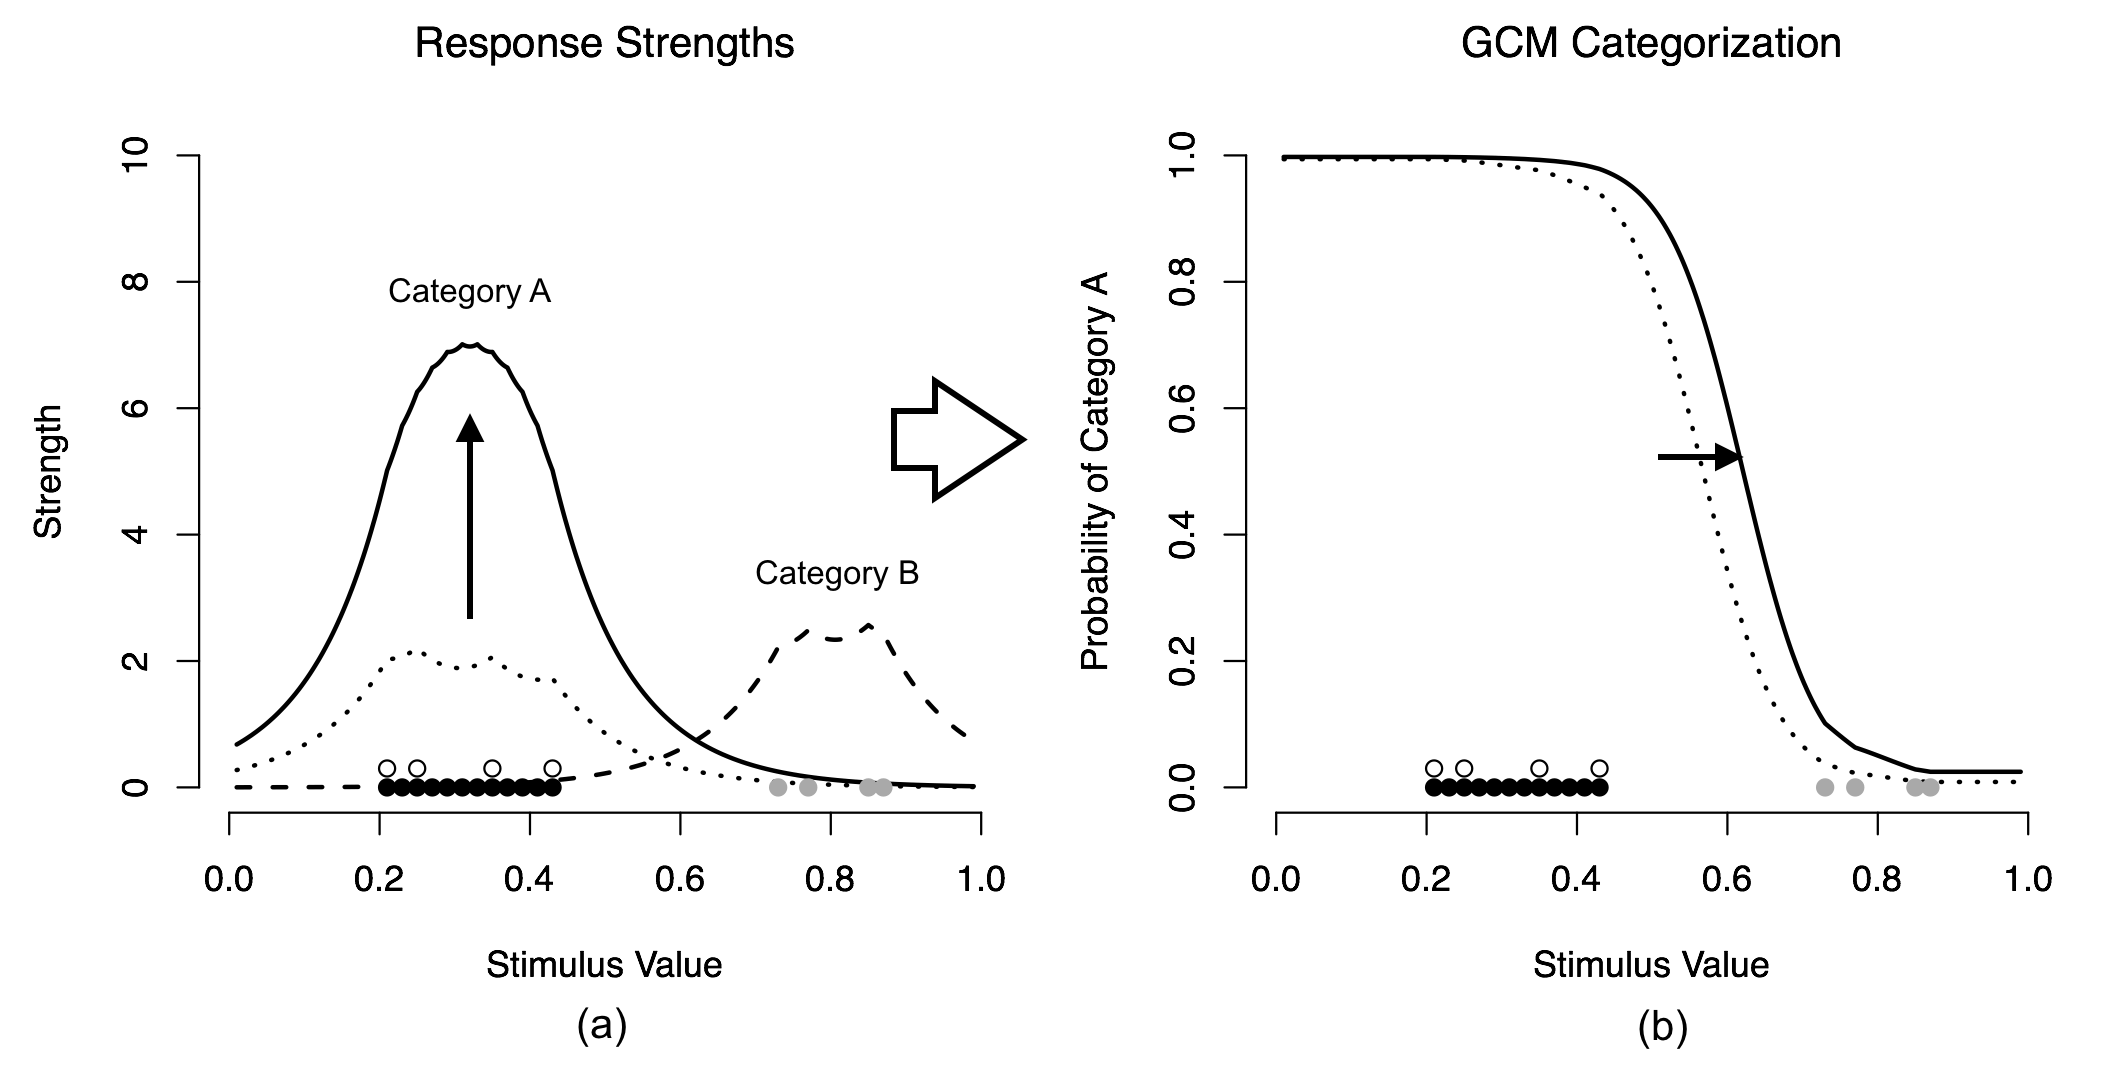
\includegraphics[scale=.35]{figures/GCM-cat.png}
\caption{The effect of sample size on the GCM in a categorization task. The left side of panel a shows how the response strength increases when the number of exemplars of a target category (category A) is increased from 4 (white markers, dotted line) to 12 (black markers, solid line). The number of exemplars of category B (gray markers) is held constant at 4, and so the response strength (dashed line) remains unchanged. The effect on categorization is shown in panel b: because the response strength for category A increases relative to category B, the category boundary expands to the right.}
\label{fig:gcmExample}
\end{center}
\end{figure}


Moreover, it should be noted that this prediction is not specific to the GCM or exemplar models. Rather, it is grossly typical of categorization models generally. For instance, prototype-hybrid models shift the prior beliefs of the category of new items to match the empirical category frequency or create new prototypes within the more frequent category \cite{anderson1990adaptive, anderson1991adaptive, sanborn2010rational, sanborn2006more, love2004sustain}. Decision-boundary models \cite{ashby1988decision, ashby1988toward, ashby1986varieties, ashby1993relations} and knowledge partitioning models \cite{lewandowsky2000knowledge, lewandowsky2000competing, yang2004knowledge} either do not change with increased frequency, or shift their representations to increase the portion of the stimulus space that corresponds to the more frequent category.
Even a Bayesian category learning model based on rule-inference will increase the complexity of the category rule with more items, leading to increased generalization for new items \cite{Goodman2008rational}.

%The characteristic of the GCM approach to categorization that matters most for our purposes is the manner in which sample size influences decision making. If new exemplars are added to category $c$, or if new instances of old exemplars are encountered, the response strength $\eta_{ic}$ for that category increases, but the response strengths for other categories remain unaffected. Consequently, the effect of adding exemplars only to one category is to {\it increase} the probability that future exemplars will belong to that category. Within the model, this claim depends on the assumption that adding observations does not induce systematic changes to GCM parameters (e.g., if $\lambda$ scales with $N$). The GCM in its standard form does not provide any theoretical reason to expect such changes, but this is an important point that we will return to later. For the moment it suffices to note that a default application of the GCM to a categorization problem does not allow the probability of category membership to decrease when new exemplars are observed from that category.


\subsection{Applying the GCM to a generalization problem}

The GCM in the form described by \citeA{nosofsky1986attention} is primarily a model for how people choose {\it which} category to assign a novel item to. Thus, although it is related to Shepard's theory of generalization, it is not itself a model for generalizing a single category.
% It provides answers the ``Dax or Wug?'' question, not the ``is this a Dax?'' question.
Nevertheless, it is not difficult to extend the GCM to make a prediction of this form, and indeed this extension was proposed by \citeA{nosofsky1991tests} not long after the GCM was originally developed. The intent at the time was to adapt the GCM to serve as a model of recognition memory. Recognition memory experiments have much the same structure as a generalization task: people are shown items that belong to a single list (the target category) and asked whether a test item was found on the study list. The two problems are not perfectly equivalent in that the recognition memory task asks for an identification decision rather than an inductive generalization, but there is mounting evidence \cite{nosofsky1991tests, hawkins2016dynamic, nosofsky2016exemplar, nosofsky2014exemplar} that the underlying processes between recognition memory and induction may be much the same. With that in mind, we suggest that the \citeA{nosofsky1991tests} model represents the natural way to adapt the original GCM to a generalization problem.

The model works in the following way. If the learner has observed multiple stimuli that all belong to the target category $c$, a response strength for that category $\eta(y,c)$ is computed using Equation~\ref{gcm2} above, with no differences from the categorization context. However, because the generalization problem does not provide a contrast category, the generalization probability is computed by comparing $\eta(y,c)$ to a threshold $\phi$:

\begin{equation}
\label{gcm4}
P(y \in c) = \frac{\eta(y,c)}{\eta(y,c) + \phi}
\end{equation}

On its face, this seems a sensible adaptation of the GCM. It retains all the core theoretical constructs that the original GCM used to solve a categorization problem, and the only novel entity is a threshold parameter that has proven successful in adapting GCM in very closely related designs. What does it predict?

The behavior of the GCM in a generalization design is plotted in Figure~\ref{fig:gcmExample2}, and unsurprisingly the effect is closely analogous to the pattern shown in Figure~\ref{fig:gcmExample}. If we increase the number of exemplars of the target category without changing the range they span, the response strength rises (panel a). As a consequence, if the threshold parameter $\phi$ is held {\it constant}, the overall effect is to push the generalization gradient (panel b) outwards, away from the observed exemplars. That being said, a little care is required: it is not clear that one should expect the threshold $\phi$ to remain constant as the number of exemplars in the target category is increased. For example, in the context of manipulating set size in recognition memory tasks, \citeA{nosofsky2011short} proposed a variant of the GCM in which the threshold scaled linearly with the number of items (i.e., $\phi$ is replaced with $m\phi$ in Equation~\ref{gcm4}, where $m$ is the number of training items). This version of the GCM makes somewhat different predictions when applied to a single-category generalization task. As we discuss later in the paper (see Figure~\ref{fig:gcmExample3}) for many parameterizations this model predicts no effect of category frequency rather than the modest expansion shown in Figure~\ref{fig:gcmExample2}, however the prediction depends on the interaction between multiple model parameters.

An important point to note at the outset is that there are almost certainly ways in which variations of the GCM could produce cateogry tightening. For instance, one very sensible possibility would be to assume that the specificity parameter ($\lambda$ in Equation~\ref{gcm1}) {\it also} increases as a function of sample size, perhaps reflecting an adaptive generalization process -- when training items cover the stimulus space more densely, the learner is less reliant on the need to generalize widely from any specific exemplar, and as such one might expect $\lambda$ to change systematically. Nevertheless, absent a substantive theory as to why $\lambda$ might change systematically with sample size in one design (generalization) and not in another (categorization), it seems reasonable to leave this open to future work. As such, for the purposes of this paper we take category expansion or no effect of category frequency to be the ``default'' predictions of the GCM in a generalization design.


%that varied based on the number of items. This model is much more flexible, and simulations using their reported best-fitting parameters produce a weaker category frequency effect than shown in Figure~\ref{fig:gcmExample2} though large values of $\lambda$ and $\phi$ can produce no effect of category frequency (Figure~\ref{fig:gcmExample3}) or even generalization tightening. Given the prediction based on the best fitting parameters of \citeA{nosofsky2011short} and a lack of theory about how $\lambda$ should change as a function of category structure -- we suggest that the {\it default} prediction of the GCM in a generalization design should be weak expansion rather than narrowing. That being said, in the discussion section we outline how to adapt the GCM, based on the principles of \citeA{nosofsky2011short}, to account for our results in generalization designs by adjusting $\phi$ and $\lambda$ as a function of category frequency as well as assumptions about the sampling process.

% DANI - I feel like a detailed discussion of the Nosofsky et al model here might produce some confusion, so I've tried to condense it. Besides, we refer the reader to the discussion anyway, so going into details here feels like we're creating problems for ourselves

%However, if the stimulus generalization parameter $\lambda$ remains fixed, the \citeA{nosofsky2011short} model consistently produces either category expansion or narrowing across all possible values of the slope and intercept of the linear relationship between $\phi$ and category frequency.

%, a prediction that is difficult to explain given the results reported here. [Drew: Is this true?]

%It should be noted that if $\phi$ is allowed to change as a function of sample size the GCM makes no prediction at all, insofar it is always possible to choose values of $\phi$ that move the generalization gradient in any direction.



\begin{figure}[t]
\begin{center}
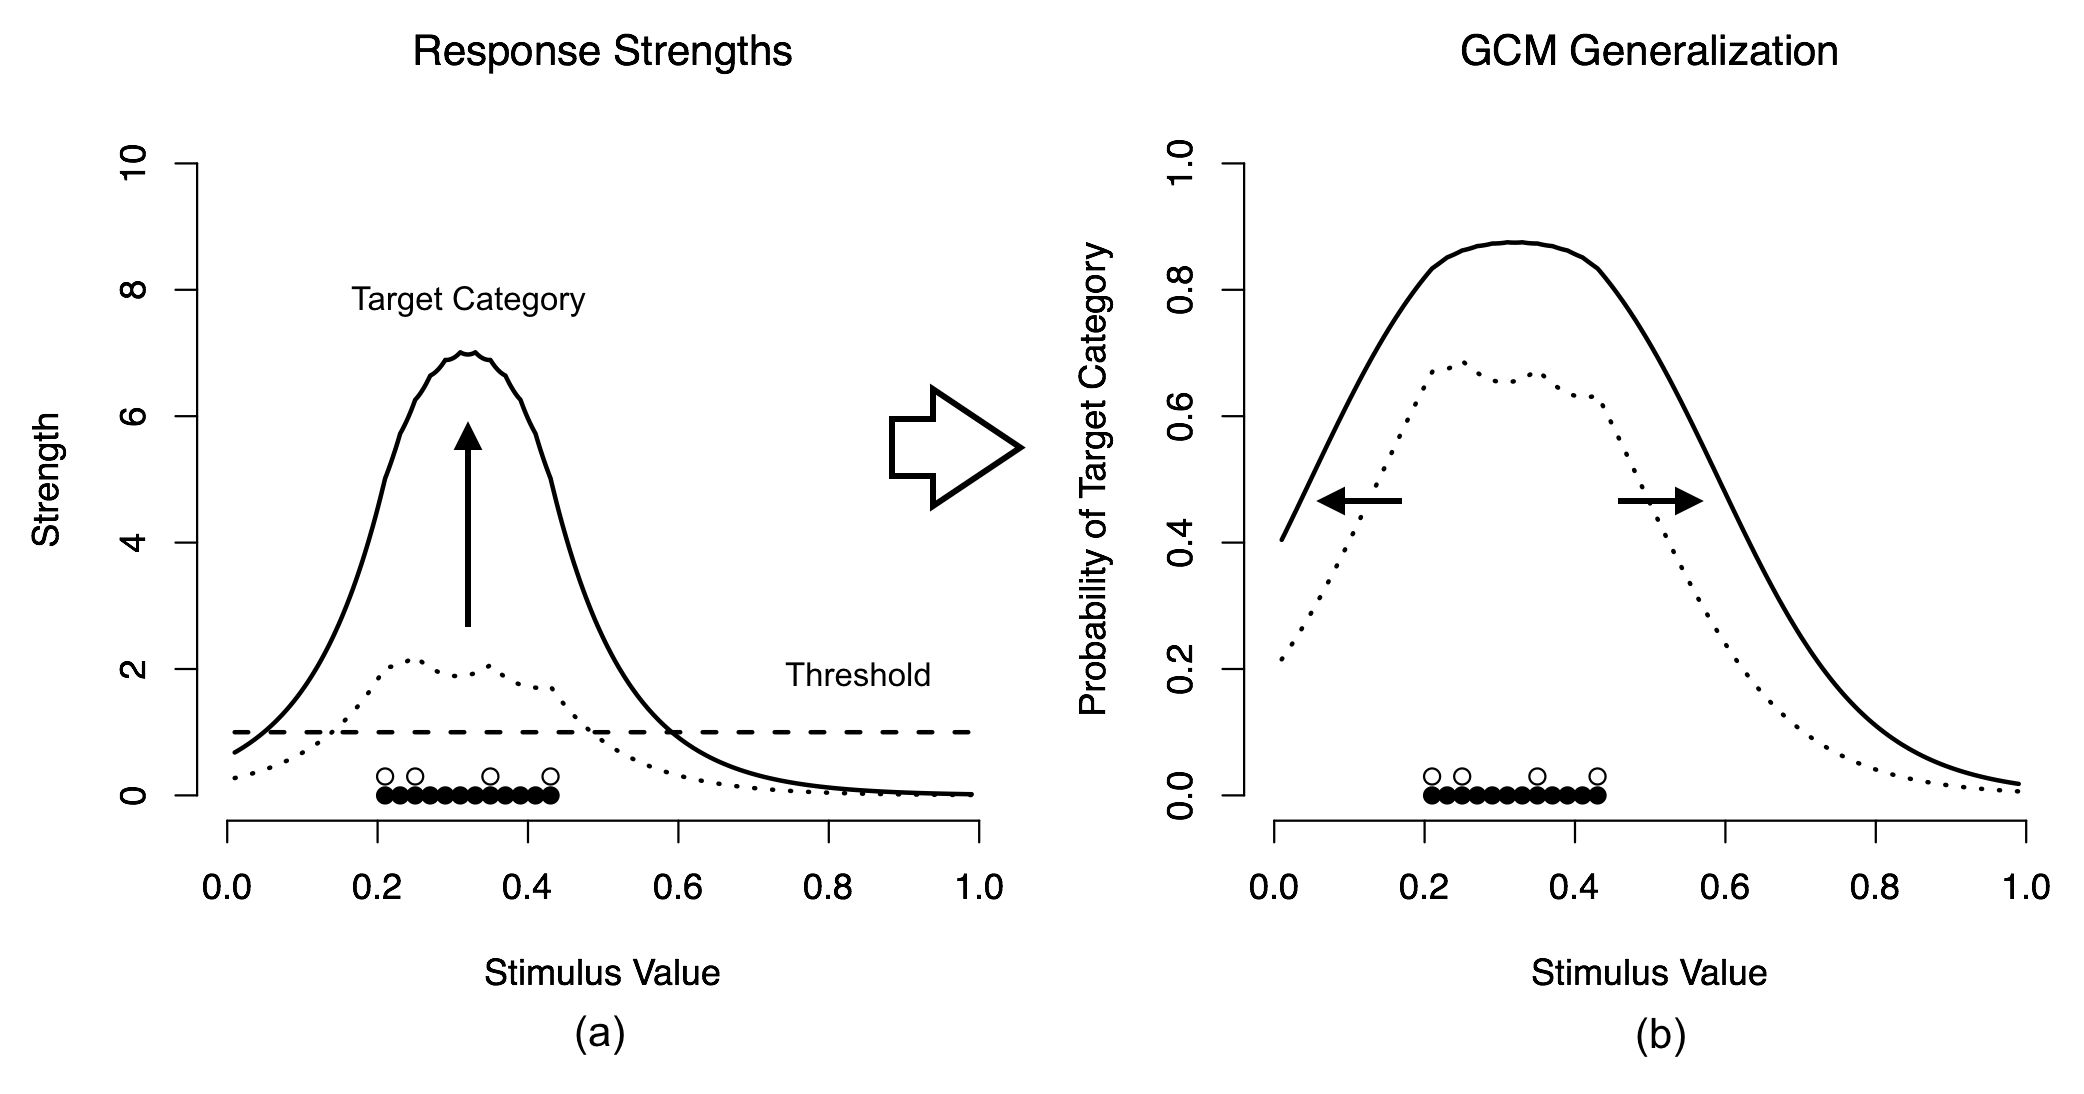
\includegraphics[scale=.35]{figures/GCM-gen.png}
\caption{The effect of sample size on the GCM in a generalization task. The response strengths for the target category are shown in panel a, and are identical to those depicted for category A in Figure~\protect\ref{fig:gcmExample}. However, because the generalization task does not present exemplars from a contrast category, the response strength is compared against a fixed threshold. The effect on generalization is shown in panel b: increasing the sample size pushes the generalization gradient outwards, away from the observed exemplars.}
\label{fig:gcmExample2}
\end{center}
\end{figure}


%Figure~\ref{fig:gcmExample} shows the predictions of the GCM when it is given exemplars from two categories, as sample size within one of those categories increases from four to twelve (without changing the overall range that the exemplars cover, of course). By convention we refer to the category with the changing sample size (and shown on the left side of the $x$-axis) as Category A, and the one on the right as Category B.The left panel shows categorization judgments, represented as choice probabilities in the model, while the right panel illustrates the resulting generalization gradients. It is clear that in both cases, the additional exemplars results in the model {\it expanding} the gradient: being more likely to accept more distant items as a member of Category A as well as more likely to generalize Category A to more distant items. In fact, unless some other parameter (e.g., $\lambda$ or $\phi$) changes systematically as $N$ increases for some externally-motivated reason, the response strength $\eta(y,c)$ {\it necessarily} increases as more exemplars are observed. The increase can be very small, but no other parameters values within this model allows the generalization probability to decrease as a function of sample size.%\footnote{That said, the parameters we used for the simulations shown are: $c=10, \gamma=1$,  }
% AP: Is there anywhere we want to say what specific values we assumed for lambda, phi, etc here? We're saying it doesn't matter but people might want to know. This could just be a footnote. And note that we did try systematically varying them (I think we did?) and showed it didn't change the qualitative prediction...


\subsection{The Bayesian model for generalization}

A different perspective on inductive generalization is suggested by the Bayesian model of \citeA{tenenbaum2001generalization}. Like the GCM, this approach can also be viewed as an extension of the work of \citeA{shepard1987universalsim} on stimulus generalization. Unlike the GCM, it is a more direct extension. This framework assumes that a learner is given a set of $N$ items $\bm{x}=(x_1,\ldots, x_N)$ that all belong in the same category. The learner's goal is to infer whether that category generalizes to include a novel item $y$.
The learner accomplishes this by constructing a set of ``consequential regions'' of the psychological space, where each possible region is a candidate hypothesis ($h$) for the consequential region that defines the category \cite<see>[for related approaches]{navarro2006natural,soto2014explaining,griffiths2012bayesian}.
The prior degree of belief $P(h)$ for each such hypothesis is updated to a posterior distribution via Bayes' rule:

\begin{equation}
\label{tg1}
P(h | \bm{x}) = \frac{P(\bm{x} | h) P(h)}{\sum_{h^\prime \in \mathcal{H}} P(\bm{x} | h^\prime) P(h^\prime)}
\end{equation}

\noindent
where $P(\bm{x} | h)$ describes the likelihood that the learner would have observed the items $\bm{x}$ if $h$ were indeed the true extension of the category. The generalization probability is then constructed by summing the posterior probabilities of those hypotheses that contain the novel item $y$:

\begin{equation}
\label{tg2}
P(y \in c) = \sum_{h | y \in h} P(h | \bm{x})
\end{equation}

\noindent
As \citeA{tenenbaum2001generalization} point out, this framing of the generalization problem includes Shepard's model as a special case, and has many connections with theories of similarity. Inference in the Bayesian generalization model is driven by the likelihood function $P(\bm{x}|h)$, which provides the mechanism for belief revision in the model. The model assumes that items are sampled in a conditionally independent manner, which allows the probability of several items $\bm{x}$ to be expressed as the product of their individual probabilities:

\begin{equation}
\label{tg3}
P(\bm{x} | h) = \prod_{i} P(x_i | h)
\end{equation}

One of the major departures from Shepard's original model lies in the way that this likelihood function is constructed. Shepard argued that a typical generalization scenario was one in which nature selects the item $x$ independently of the consequential region $h$, yielding what has been termed a ``weak sampling'' model \cite{tenenbaum1999bayesian}. This weak sampling model does not change the relative belief assigned to any hypothesis based on the number of items that belong in the category. However, Shepard's weak sampling model is untenable in a situation when {\it many} items are all constrained to belong to the same category. Given this, \citeA{tenenbaum2001generalization} make the simplest possible alteration to Shepard's assumption of independence: their ``strong sampling'' model assumes that items are sampled such that they are constrained to belong to the relevant category but are otherwise chosen uniformly at random. This slight change introduces a dependency in the likelihood function on the structure of the hypothesis. Specifically, if the hypothesized category has size $|h|$, then this means that the likelihood function becomes:

\begin{equation}
\label{strongSampling}
P(x_i | h) = \left\{ \begin{array}{lr} 1/|h| & \mbox{ if } x_i \in h \\ 0 & \mbox{ otherwise} \end{array} \right.
\end{equation}

In one sense the shift from weak sampling to strong sampling is trivial: it merely incorporates a sensible constraint imposed by the fact that the generalization problem now can incorporate multiple items from the same category. However, it entails a very non-trivial consequence known as the {\it size principle}: as the sample size $N$ increases, the probability of small hypotheses will increase relative to larger hypotheses
\cite{tenenbaum1999bayesian}. To see why this holds, consider the relative degree of belief that the learner has in two hypotheses $h_1$ and $h_2$ after observing $N$ items. Assuming that both hypotheses are consistent with all the observations, then:

\begin{eqnarray}
\label{tg4}
\frac{P(h_1 | \bm{x})}{P(h_2 | \bm{x})}
&=& \frac{P(h_1)}{P(h_2)} \times \prod_{i=1}^{N} \frac{P(x_i | h_1)}{P(x_i | h_2)} \nonumber \\
&=& \frac{P(h_1)}{P(h_2)} \times \prod_{i=1}^{N} \frac{1/|h_1|}{1/|h_2|} \nonumber \\
&=& \frac{P(h_1)}{P(h_2)} \times  \left( \frac{|h_2|}{|h_1|} \right)^N
\end{eqnarray}

\noindent
Unlike a learner that assumes weak sampling and has no preference based on hypothesis size, if the two hypotheses are different sizes, the learner who assumes strong sampling will come to prefer the smaller one. Moreover, the extent of this preference grows exponentially larger as the sample size $N$ increases. The net result of increasing the sample size is that the learner shifts belief from large hypotheses to small ones and the generalization gradient tightens. This effect is depicted visually in Figure~\ref{fig:bayesExample}. The tightening of generalizations with increased samples is a direct result of assuming strong sampling, a fundamental characteristic of this model.
While there are a number of ways in which the model could be adapted by modifying the hypothesis space, the prior, or the sampling model, the ``default'' prediction of the Bayesian generalization model is very different to the prediction we arrive at by adapting the GCM to generalization problems.



\begin{figure}[t]
\begin{center}
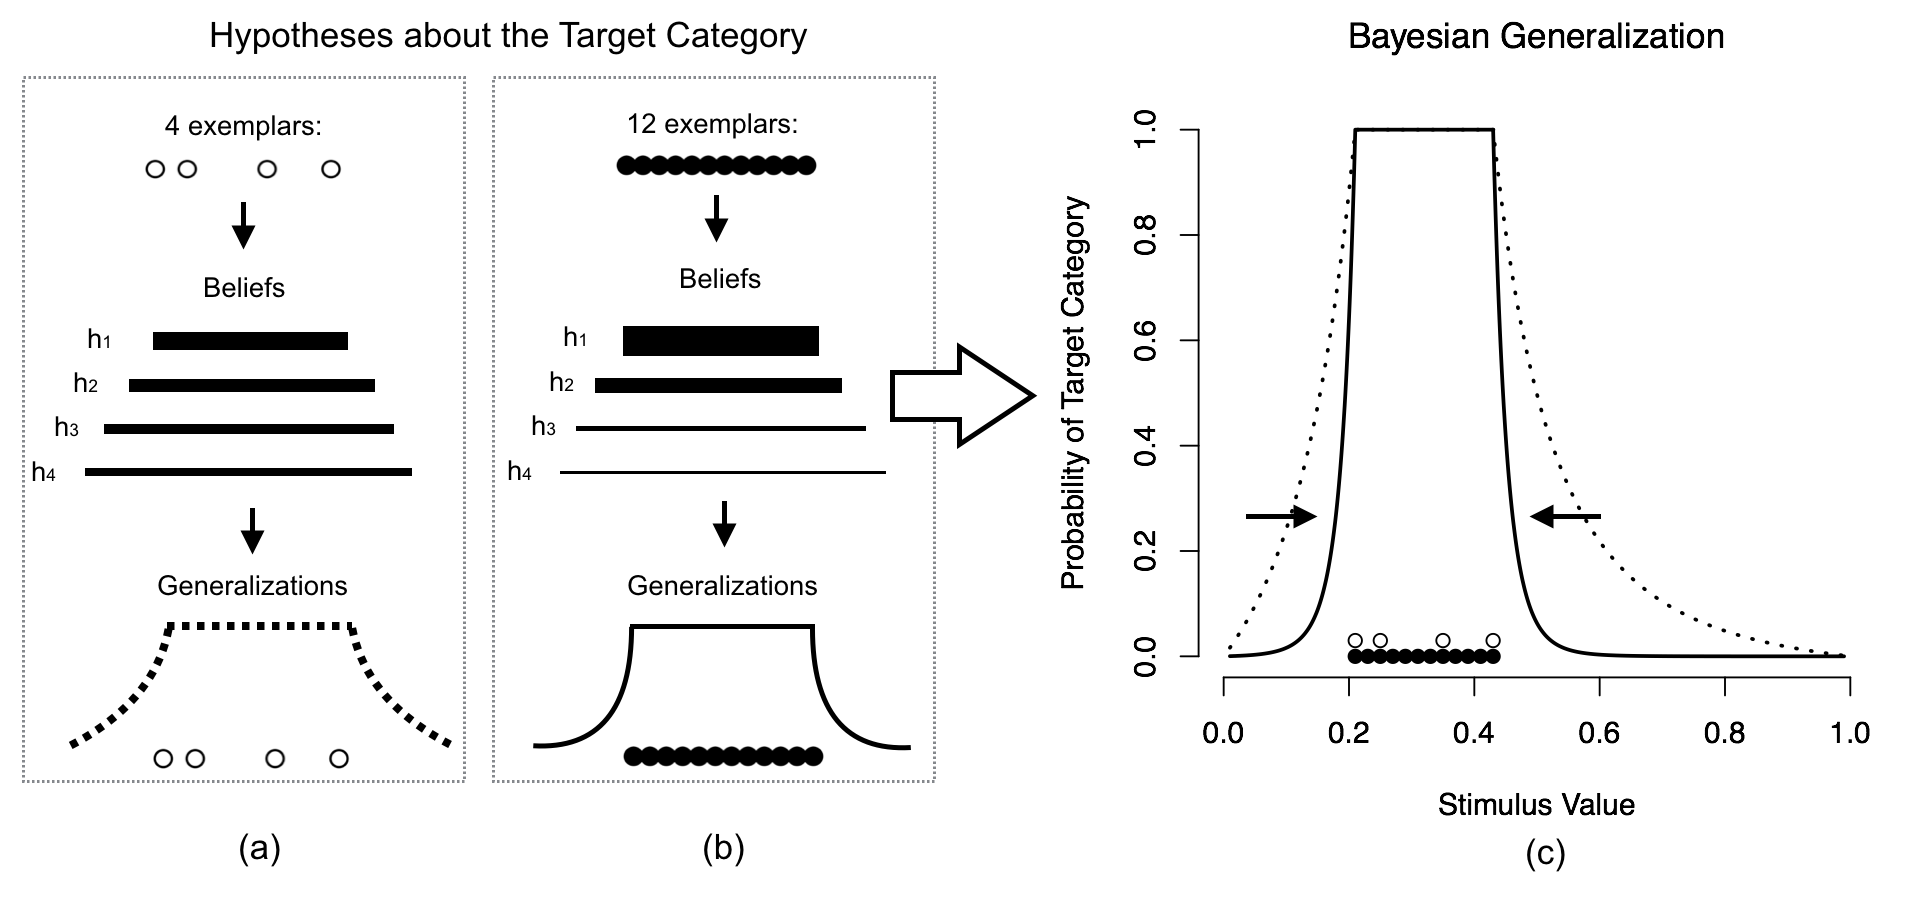
\includegraphics[scale=.4]{figures/Bayes-gen.png}
\caption{The effect of sample size on the Bayesian generalization model in a generalization task. In the case of observing 4 exemplars drawn from a target category (top of panel a), it is plausible to think that the true extension of the category might be much broader than the range spanned by those items. Illustrating this idea, the middle of panel a shows the relative degree belief in four hypotheses (horizontal lines), where the width of each line reflects the amount of belief in that hypothesis. By averaging over their beliefs about the hypothesis (bottom of panel a) the learner obtains a broad generalization gradient. In the case of 12 exemplars that span the same consequential region (as in panel b) this evidence very strongly favors smaller hypotheses, producing more belief in smaller hypotheses and thus narrower generalization gradients. Panel c show the generalizations made by a Bayesian learner who considers all possible intervals defined over a finite range for the 4 and 12 exemplar cases (see Navarro, et. al., 2012, for analytic expressions).}
\label{fig:bayesExample}
\end{center}
\end{figure}

\begin{figure}[t]
\begin{center}
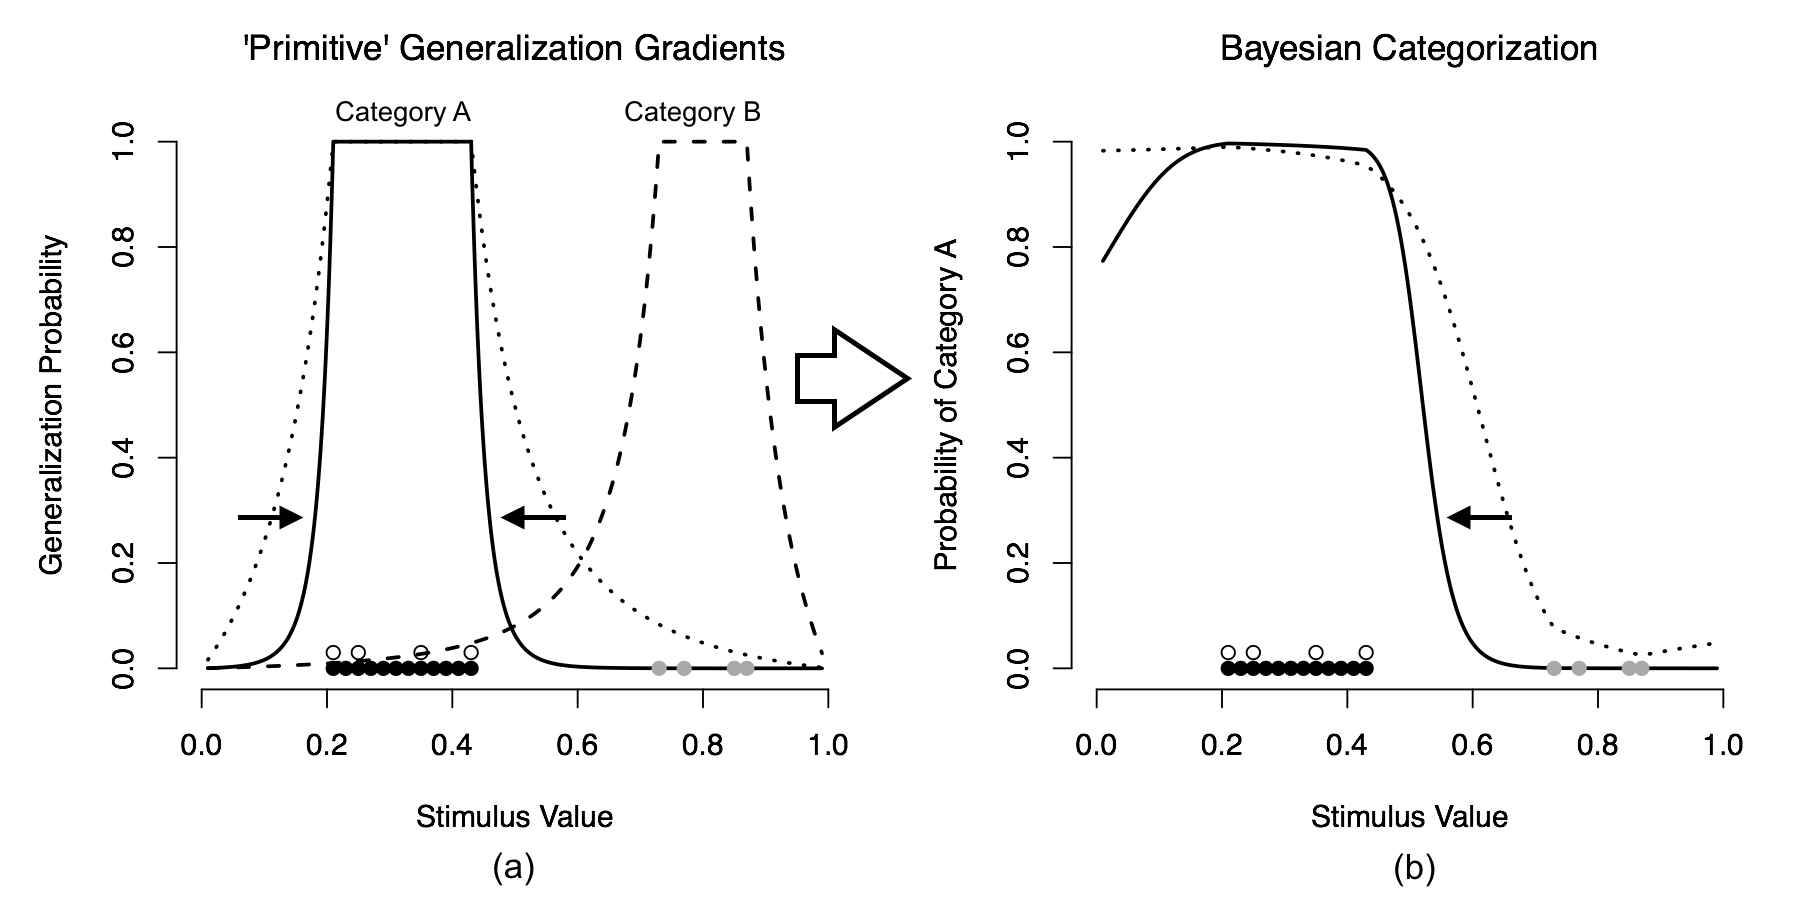
\includegraphics[scale=.4]{figures/Bayes-cat.png}
\caption{The effect of sample size on the Bayesian generalization model in a categorization task. Panel a shows the ``primitive'' generalization curves that result from the learning about the extension of each category by applying the strong sampling model to each category independently. Even when combined with a mechanism for learning the different frequencies of the two categories (Equation~\ref{tgadapt2}), the overall result produces a shift in the category boundary closer to category A when the sample size is increased (panel b).}
\label{fig:bayesExample2}
\end{center}
\end{figure}


\subsection{Applying the Bayesian generalization model to categorization}

Though originally conceptualized in terms of finding the consequential regions for a {\it single} category, it is not too difficult to extend the Bayesian generalization model to two or more categories, and there is at least some empirical evidence suggesting that the framework can be fruitfully applied to multiple-category tasks \cite{vong2013role}.

How should we determine default predictions for the Bayesian generalization model in a categorization task? As was the case with the GCM, there are multiple ways in which the Bayesian generalization model can be adapted to a categorization problem. In our view, the most transparent way to do this is to treat the generalization gradients from each category as if they were ``primitive'' entities that drive the categorization decisions. That is, the generalization probability for each category forms the {\it response strength} associated with that category, and the choice probability is proportional to this response strength \cite{luce1959individual}. Formally, if the positive examples for each category are modeled as an independent Bayesian generalization process, the posterior estimates can be combined without regard to the frequency of each category as in the decision rule for the GCM (Equation~\ref{gcm3}):

\begin{equation}
\label{tgadapt1}
P(l_y = c) =  \frac{P(y \in c)}{\sum_{c^\prime} P(y \in c^\prime)}
\end{equation}

\noindent
where $P(y \in c^\prime)$ describes the generalization gradient inferred for category $c^\prime$ using Equation~\ref{tg2}. As the number of items in category $c$ increases and the generalization gradient $P(y \in c)$ tightens, the category boundary will also tighten.
% For a categorization design, a natural analog of strong sampling is a model that (at a bare minimum) requires all items to belong to one of the $K$ categories under consideration: one does not expect to observe a zebra in an experiment asking participants to classify dogs.

Nevertheless, this is not the only way to make this adaptation. For instance, one might construct versions of the model that make different assumptions about the hypothesis space or sampling assumption. For the purposes of this paper, however, we wish to hold these assumptions constant to the greatest possible extent, in order to determine what the Bayesian generalization model would predict about categorization tasks, if there were no ``deep'' differences between the tasks. A (somewhat) principled way to do this is as follows. Exemplars are sampled such that a category label is selected at random (with some unknown probability associated with each label), and then an exemplar from that category is selected uniformly at random, which is necessary to preserve the strong sampling assumption of the model. The hypothesis space for this model assumes that the consequential regions associated with each category are {\it independent} -- an exemplar can belong to one or both of the categories, or neither. This permits the category representations to be separate from the nature of the response task, allowing ratings of a single category probability in {\sc probability} response tasks, binary classification in {\sc forced choice} tasks, or `none of the above' category responses when permitted \cite{navarrosubmittednone}.
%, and it is only due to the forced choice nature of the categorization task, which forbids ``none of the above'' responses, that the response is binary \cite<but see>{navarrosubmittednone}.
As shown in the Appendix, this yields an alternative form for Equation~\ref{tgadapt1}:

\begin{equation}
\label{tgadapt2}
P(l_y = c) =  \frac{P(c) P(y \in c)}{\sum_{c^\prime} P(c^\prime) P(y \in c^\prime)}
\end{equation}

\noindent
where the inferred prior probability $P(c)$ for category $c$ is related to the number of times the category has been observed.

The predictions about sample size that emerge from Equation~\ref{tgadapt2} are somewhat less obvious than Equation~\ref{tgadapt1} because there are two different mechanisms involved: as described before, the generalization gradients $P(y \in c)$ tighten exponentially as the category frequency increases, causing the category boundaries to {\it contract} towards the category. However, this effect is somewhat offset by the fact that the prior probability of the label $P(c)$ {\it increases} linearly with frequency, causing boundaries to {\it expand} away from the category. Nevertheless, as Figure~\ref{fig:bayesExample2} shows, the exponential tightening dominates the linear expansion and the overall effect of increasing category frequency in Equation~\ref{tgadapt2} results in tightening for the category boundary. Thus, mirroring what we observed with the GCM, when we extend the Bayesian model of generalization to a categorization problem -- while holding the sampling assumption and hypothesis space associated with the categories unchanged -- we arrive at a model that makes the opposite ``default'' prediction about sample size to the one made by the GCM.

\subsection{How should we interpret the discrepancy?}

The inconsistency between these models is striking enough on its own, but becomes even more surprising when one recognizes that the GCM is known to make good predictions about how frequency information is used in categorization \cite<e.g.,>{nosofsky1991tests, nosofsky1988similarity}, and that the Bayesian strong sampling model makes accurate predictions in inductive generalization tasks \cite<e.g.,>{ navarro2012sampling, xu2007word}. Each model correctly captures the empirical pattern in its own domain, yet when the central principles of both models are extended to the other domain -- without making any special claims that something is different about generalization and categorization -- they make the opposite prediction to each other. If this is true, it suggests that generalization {\it decreases} as experience of a category increases, but the probability of assigning items to that category {\it increases} with more observations. This is, to put it mildly, puzzling.

Why does this inconsistency occur? One somewhat dispiriting possibility is that the empirical evidence for one (or both) of the effects is simply wrong. Alternatively, it is possible that both effects are real but are dependent on superficial properties of the task.
One especially plausible possibility is that the source of the difference lies in the choice of dependent measure. Most categorization experiments use a forced-choice response while nearly all generalization experiments ask people to rate the probability of category membership. Though it is not obvious why this should drive different changes due to sample size, it is nevertheless a major difference between experiments that produce an expansion in categorization \cite<as exemplified by, e.g.,>{nosofsky1988similarity} and those that produce tightening effects in generalization \cite<as exemplified by, e.g.,>{navarro2012sampling}.

A more interesting possibility is the suggestion that there are {\it systematic} differences between the inductive problems posed by categorization and generalization tasks, and those explain the divergent patterns of results. Perhaps the mere fact that a generalization experiment presents people with positive examples of a target category whereas a categorization experiment displays examples of multiple categories is genuinely sufficient to produce a qualitative reversal in people's inductive inferences. Our discussion of the GCM and the Bayesian generalization model hints that this might be true, simply by virtue of the fact that Figures~\ref{fig:gcmExample} and \ref{fig:bayesExample} both look like ``sensible'' models, but something seems to have gone awry with the model construction in both Figures~\ref{fig:gcmExample2} and \ref{fig:bayesExample2}. The ``minimalist'' adaptations that we have made to the GCM and the Bayesian generalization model both feel somewhat wrong for the problem they are ostensibly solving.

These considerations suggest that a head-to-head comparison between a categorization task and a generalization task is required, taking care to keep everything else constant. In the experiments below, participants learned categories with different numbers of observations (either four or twelve, as in the simulations above). The measure of interest is whether their judgments expanded or tightened with the additional observations.
Thus, Experiment 1 investigated inference when shown two categories, while Experiment 2 explored inference for one category. Within each experiment, we manipulated the task, asking separate participants either a forced-choice question about which category a novel item belongs to or a probability judgment question about how likely the novel item is to belong to the category. All other factors (e.g., nature of the stimuli, cover story, etc) were kept constant.

Our results indicate that the sole important factor is the number of categories. In Experiment 1, where there are two categories, people's judgments {\it expand} regardless of the question they were asked. This behavior is predicted by the GCM but not the Bayesian generalization model. Conversely, in Experiment 2, with one category, people's judgments {\it tighten} regardless of the question asked. This behavior is predicted by the Bayesian generalization model but not the GCM.
In Experiment 3 we explore the possibility that these changes are caused by learners making different assumptions about the sampling process in the one- and two-category tasks. The effect of category expansion in the two-category task is replicated; however, a cover story manipulation of sampling assumptions is sufficient to eliminate this category expansion effect.
We conclude with a discussion of what these results indicate about how categorization and generalization differ, and why the one-to-two-category shift should matter.

\section{Experiment 1: Categorizing objects into two categories}

\subsection{Method}

\subsubsection{Participants}

We recruited 500 participants on Amazon Mechanical Turk and collected data from 499 participants (the data from one participant was not saved). Of the 499 total participants,
23 were excluded because they had previously participated in similar online experiments run by our lab. An additional 94 were excluded for failing to meet a predefined accuracy threshold for non-critical test stimuli, described below. The remaining 382 participants were included in all analyses. Participants ranged in age from 18 to 79 (mean 32.6) with 43.5\% being female. 72.0\% of participants came from the USA, 23.6\% from India, and all other countries less than 1\%. People were paid \$0.50 for their participation in the 8-minute experiment.

\subsubsection{Design}

Participants were randomly assigned to one of four conditions in a 2x2 between-subjects design. The first factor varied the number of exemplars from Category A that the participants were shown, either {\sc four} (N=209) or {\sc twelve} (N=173). Category B consisted of four exemplars regardless of condition. The second factor manipulated the response elicitation method: people were either  asked to provide {\sc forced choice} decisions in which they had to assign a novel item to Category A or Category B (N=228), or they were asked to rate the {\sc probability} that the novel item belonged to Category A (N=154).



\begin{figure}[ht]
\centering{
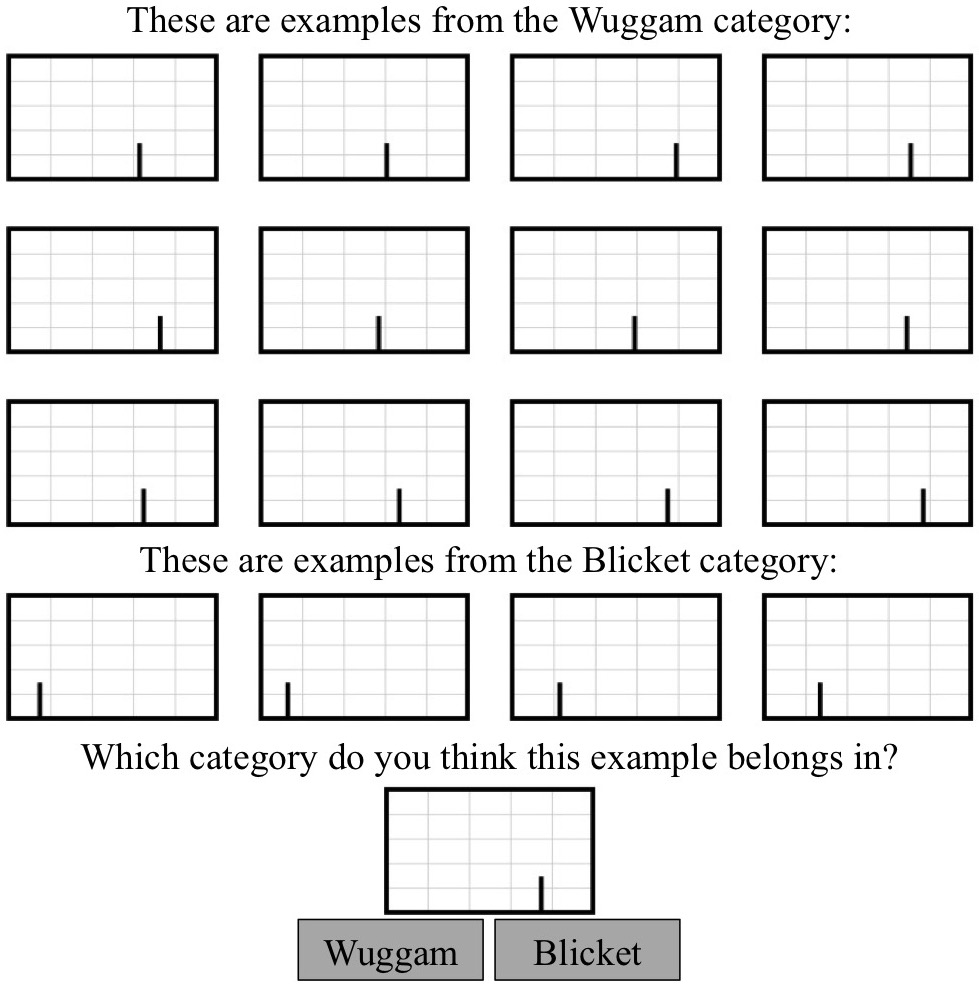
\includegraphics[width=4in]{figures/two-category-screenshot.jpg}
\vspace*{12pt}
\caption{Sample stimulus display used in the two-category task (Experiment 1). The twelve training stimuli from Category A (labeled Wuggams) are in the top three rows, with the four stimuli from Category B in the fourth row. The single test exemplar from this trial is shown at the bottom of the figure along with two response buttons.
The {\sc probability} condition looked identical except that instead of two buttons at the bottom people saw a slider with values ranging from 0\% to 100\% and a submit button.}
\label{fig:two-category-screenshot}
}
\end{figure}


\subsubsection{Stimuli}

Stimuli consisted of an outer rectangle that was 185 pixels wide and 110 pixels tall, with a vertical black line drawn on the interior of the rectangle. To assist people in making perceptual discriminations four evenly-spaced light gray vertical and horizontal grid lines were included within each rectangle. Example stimuli are shown in Figure~\ref{fig:two-category-screenshot}.

Categories were defined in terms of the values along only one dimension, but the nature of the dimension was randomly varied between participants: for some, the black lines varied by position, and for others, they varied by height. Stimuli were also left-right reversed for a random half of the participants. All analyses collapse across both of these factors, as none of them materially affected the conclusions.

Each stimulus varied along the one relevant stimulus dimension; we refer to this as the \textit{value} of the stimulus. The value for line height varied from 5\% to 95\% of the height of the rectangle, and the value for line position varied from 5\% to 95\% of the width of the rectangle from the left edge.
For clarity of exposition, we describe the rest of the experiment in terms of the condition in which the dimension varies by position and Category B values are encoded with higher numbers, even though both of these factors were completely randomized in the actual experiment.

Stimulus values were defined to match the values in the simulations in Figures~\ref{fig:gcmExample} and \ref{fig:bayesExample}. Category B, which was identical for all participants, contained four stimuli (as in the fourth row of Figure~\ref{fig:two-category-screenshot}) with values of 73\%, 77\%, 85\%, and 87\%. For all participants, the range of values in Category A were identical, spanning from 21\% to 43\%. Participants in the {\sc twelve} condition observed all of the odd-numbered stimulus values within that range in addition to these endpoints, resulting in twelve exemplars total. Those in the {\sc four} condition saw an additional two values randomly selected from between the endpoints, making four total.



\subsubsection{Procedure}

Participants were told that they were going to be shown a few example objects from two categories and then asked to make judgments about new objects while the examples remain on the screen. Participants making {\sc probability} response judgments were instructed to ``indicate how likely you think it is that this object belongs in the specified category.'' Participants making {\sc forced choice} responses were instructed to ``indicate which category you think this object belongs in.'' Both conditions were required to answer a series of three check questions designed to make sure they understood the instructions and then proceed to a training and test session. Those that did not answer all of the questions right were returned to the instructions until they did.

%\footnote{Full instructions for the probability judgment condition: In this task you will be asked to indicate how likely it is that objects belong in one of two categories. All of the objects you will see consist of a black line within a black box that has a grey background pattern. The only differences between objects involve the line within the box. When you start the task you will be shown a few example objects from each category. Please take the time to study these examples and then press the Next button. After pressing Next, you will be shown a new object and asked to indicate how likely you think it is that this object belongs in the specified category. The existing examples of both categories will still be present on the screen and you can compare the new object to the examples. To indicate your guess select the response option that most closely matches how likely you think it is that the object belongs in the specified category. When you are happy with your guess, press the Next button to record your response and proceed to the next object. You will be asked to judge 19 objects in total, please do not rush through these judgments. After these judgments you will be done with the task. All of the objects you will see and make judgments about are very similar and the only differences between objects involve the line within the box. Please pay close attention and take your time to spot the differences between objects. In the next section you will be asked a few questions about these instructions to verify you read and understand them. Please press Next if you are ready to proceed to the instruction checks.}
%AP: check these exact instructions
% DH: updated.

{\it Training}. Training for Category A and B was simple and identical across all four conditions. In it, people saw exemplars from two categories defined according to a one-dimensional feature as described above. All of the stimuli appeared immediately, some as exemplars of Category A and some as exemplars of Category B, as in Figure~\ref{fig:two-category-screenshot}. The stimuli in each category were arranged in a random order and each person saw a different assignment of two labels (Blicket and Wuggam) to the two categories. During the instructions people were told to ``When you start the task you will be shown a few example objects from each category. Please take the time to study these examples and then press the Next button.''

{\it Testing}.  In order to minimize effects of memory, all training stimuli stayed on the screen for the duration of the test phase, which was very similar regardless of what question condition people were in. In all conditions, the set of test stimuli consisted of 19 exemplars that spanned the whole range of the stimulus dimension from 5\% to 95\% in steps of 5\%.\footnote{Due to a coding error, one of the extreme stimuli (either 5\% or 95\%) was not shown to 151 participants. Neither of these stimuli were within the critical region that we focus our analysis on.} The test stimuli were shown one at a time and in a random order. The next stimulus was shown directly after participants submitted their response by pressing a button.

What question people were asked during test varied by question condition. Those in the {\sc forced choice} condition were asked ``Which category do you think this example belongs in?'' and were then presented with two response buttons, one for each category. Those in the {\sc probability} condition were asked ``How likely is it that this example is in the [Blicket/Wuggam] category?'' and were then shown 21 radio buttons with labels going from 0\% to 100\% in steps of 5\%. People in the {\sc probability} condition were always asked about the Category A label, as is typical in generalization experiments. In order to allow scope for capturing graded responding in the {\sc forced choice} condition, each test stimulus was presented once in the {\sc probability} condition and four times in the {\sc forced choice} condition. The conditions took similar amounts of time to complete.



\subsection{Results}

As mentioned above, 94 of the initial 499 people are excluded from the analysis for failure to achieve an accuracy threshold at test. This threshold was defined before analyzing any data and captured the intuition that if they understood the task and were trying, they should classify any stimulus with values between 21\% and 43\% as Category A (since that is the range of actually observed stimuli). One would expect that any stimuli with these values would be classified as A nearly 100\% of the time, but in order to be as conservative as possible we set a threshold of 80\%: those who classified the within-A items as not-A at least 20\% of the time are excluded from the analysis (setting the threshold slightly higher or lower does not materially affect the results).

\begin{figure}[t]
\begin{center}
\begin{tabular}{cc}
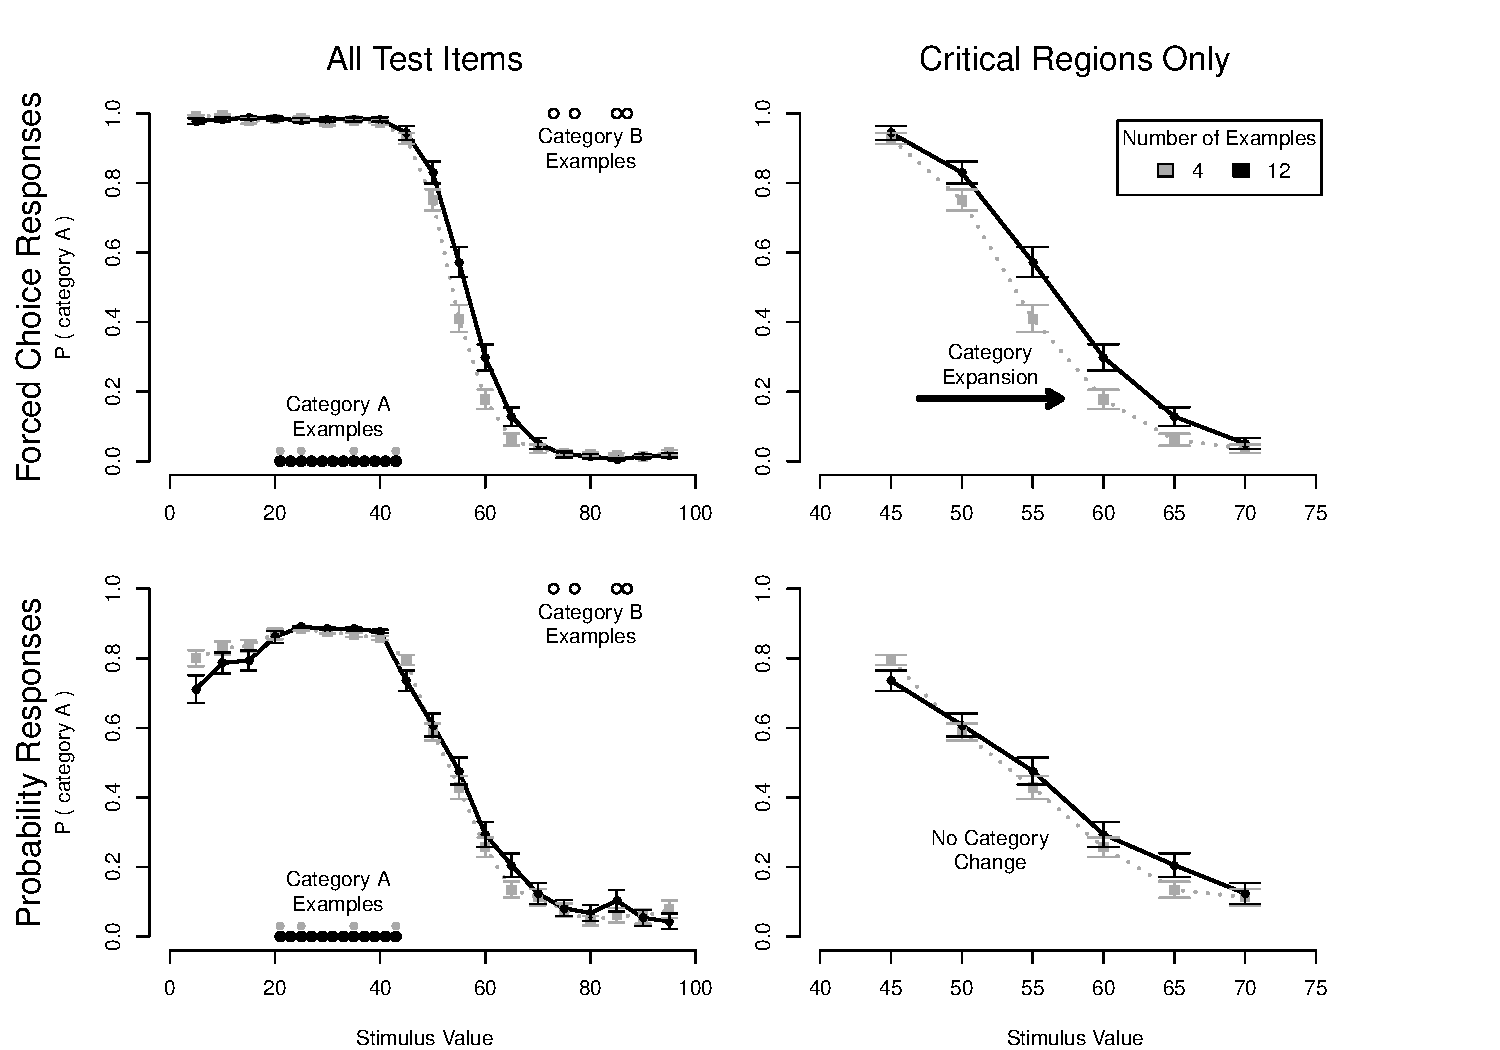
\includegraphics[width=5in]{figures/two_cat_results.pdf}
\end{tabular}
%\vspace{4mm}
\end{center}
\caption{{\small Human performance in the two-category experiment (Experiment 1). The top row shows the {\sc forced choice} condition: the proportion of answers selecting Category A in response to the question ``Which category do you think this example belongs in?'' for each possible stimulus value at test. The bottom row shows the {\sc probability} condition: the overall probability that the test item was rated as being in Category A. The graphs on the left show responses over the entire range of stimulus values; the right panels show responses for the critical range between the two categories. Points along the grey line indicate responses after seeing {\sc four} exemplars; the black points indicate responses after {\sc twelve}. Participants who saw more observations in Category A {\it expanded} their responses away from Category A, especially in the {\sc forced choice} condition. This is consistent with the predictions of the GCM but not the Bayesian model of generalization.}}
\label{fig:exp1results}
\end{figure}

The left column of Figure~\ref{fig:exp1results} shows participant responses during the test phase for all stimulus values, with the top row showing performance in the {\sc forced choice} condition and the bottom row showing performance in the {\sc probability} condition. The overall pattern is consistent across conditions, with people more likely to correctly indicate that lower stimulus values are consistent with Category A and higher values are consistent with Category B. That said, the question of whether their responses are expanding or tightening with additional exemplars is only answerable upon examination of the critical stimulus values {\it between} the categories, shown in the right column of Figure~\ref{fig:exp1results}. In both cases, especially in the {\sc forced choice} condition, there is a slight expansion away from Category A with additional training stimuli. Is this a statistically robust result?

To answer this question we compute a set of Bayes Factors that compare the relative posterior odds of three linear models.
In the \valueonly\ model, category A responses are predicted based
on the stimulus value only. In the \valuenumber\ model, predictions are based on
both stimulus value and the number of category A exemplars that participants
observed. Lastly, the \interaction\ model extends the \valuenumber\ model with a
term that models an interaction between the two predictors.\footnote{We also ran a model containing only a random intercept for each individual. The \valueonly\ model was strongly preferred over the intercept only model ($ BF > 10^{265} : 1 $) so we abandon any further comparisons involving the random-intercept-only model. All of the models also contain a random intercept for each individual. They were fit using the default parameters \cite{rouder2012default, liang2008mixtures} from the BayesFactor package (version 0.9.12-2) in R (version 3.3.1). The two predictor variables, stimulus value and the number of training examples, were coded as categorical variables.}
The data evaluated within these models consists of the critical stimulus values (45\% to 70\%, right column in Figure~\ref{fig:exp1results}), with the two question conditions ({\sc probability} and {\sc forced choice}) analyzed separately.

We first consider performance in the {\sc forced choice} condition. Logically speaking, we are interested in evaluating the impact of three different factors on whether people define a stimulus with a given value as a member of Category A or not. As a sanity check, we should expect that {\bf stimulus value} should have an impact on these judgments; people should be more likely to classify a stimulus located at 45\% as Category A rather than one at 70\%. The main variable of interest is whether the {\bf number} of observations in Category A also plays a role in determining how people categorize the stimulus. We are also interested in whether there is an {\bf interaction} between these two variables.

Table~\ref{tab:expt1bayesfactors} shows the Bayes Factors (BFs) for each of those three models, with the model including only stimulus value as the baseline. Thus, the ratio reported for each model in the table reflects the BF for that model compared to the model containing only stimulus value as the predictor.
%\footnote{For all experiments the analyses were conducted in R (version 3.3.1) using the default prior values in the BayesFactor package (version 0.9.12-2) \cite{rouder2012default}. Stimulus value and the number of training examples are coded as categorical predictor variables and a random intercept is included for each participant in all models.}
For the forced-choice judgments, it is evident from the table that the most preferred model is the one that contains both stimulus value {\it and} the number of observations as predictors. This is evidence that people did in fact change their categorization probability when Category A had more observations in it. We can estimate how much this changed by examining the posterior estimates of the parameter values from the preferred model. They suggest that the eight extra training examples lead to a 7.4\% increase in the probability of selecting Category A (95\% CI: 2.5\% to 12.5\%) for test items between the two categories. This expansion in choice probability is consistent with the predictions of the GCM and not the Bayesian model.
% AP: Is this CI correct? seems rather large especially by comparison to the other one
% DH: The values are updated and will slightly change with each resampling from the model, but this version also shows roughly the same variability. I assume the larger variability in the CI is due to something like the data being more variable. I'm happy to look into it further if needed.

\begin{table}[t]
  \centering
  \begin{tabular}{ccccc} % column spec
    \toprule
    Condition & Best Model & & Model Performance & \\
    \cmidrule(lr){3-5}
    & & Value Only & Value + Number & Interaction \\
    \midrule
    Forced Choice & Value + Number & $ 1 : 1 $ & $ \mathbf{7.6 : 1} $ & $ 6.2 : 1 $ \\
    Probability & Value & $ \mathbf{1 : 1} $ & $ 0.17 : 1 $ & $ 0.013 : 1 $ \\
    \bottomrule
  \end{tabular}
  \vspace*{12pt}
  \caption{Comparison of how well three different regression models capture human performance in the two conditions in Experiment 1. All models are linear regression models with a random intercept for each individual. We consider three nested models: predictions based on stimulus value only, stimulus value and the number of observations, and one with both predictors as well as an interaction term. In the {\sc forced choice} condition, the preferred model is the one with both stimulus value and number of observations as predictors. This suggests that, in keeping with the GCM, people were more likely to classify an item as a member of Category A if there were more observations in Category A. In the {\sc probability} condition, the preferred model did not contain the number of observations. This suggests that probability judgments do not expand with category size in the same way (although the trend was still in that direction, rather than towards tightening).}
  \label{tab:expt1bayesfactors}
\end{table}


The pattern of responses for participants in the {\sc probability} condition also shows a qualitative category expansion trend, but no evidence of a difference due to category frequency. As Table~\ref{tab:expt1bayesfactors} shows, performing the same model comparison as before ends up favoring the model whose only predictor is stimulus value. In other words, the number of observations did not have a significant effect on people's answers to the probability judgment question. That said, the trend is also in the direction of category expansion and not category tightening. This matches the posterior estimates of the parameter values from the model that includes number of observations which show that the eight extra training examples lead to a 2.0\% increase in probability judgment (95\%CI: -3.3\% to 7.2\%).

\subsection{Discussion}

The results from Experiment 1 are ambiguous in one sense, but very clear in another. It is not entirely clear whether an expansion effect was observed for both the {\sc forced choice} and {\sc probability} judgment tasks: taken at face value the results suggest an effect exists when people are asked to make force choice decisions, but disappears when asked to give probability judgments.
However, it is clear that there is no evidence for the category tightening effect predicted by the Bayesian model and shown in Figure~\ref{fig:bayesExample2}. The results are far more compatible with the GCM predictions shown in Figure~\ref{fig:gcmExample}.
% While it might genuinely be the case that people categorize differently depending on the response measure, a more plausible explanation is that there is a weak category expansion effect regardless of the measure but forced choice judgments are more sensitive to changes than probability judgments.

% This ambiguity notwithstanding, one thing is very clear:

%%%%%%%%%%%%%%%%%%%%%%%%%%%%%%

\section{Experiment 2: Generalizations about one target category}

The superior performance of the GCM on a categorization task raises the possibility that it might also outperform the Bayesian approach on a generalization problem. Perhaps previous papers that found a tightening effect in generalization were false positives, or perhaps differences in experimental procedure can account for the difference in results. With this in mind, we conducted a second experiment in which people were shown examples from one category and asked to make generalizations about new items, but in every other respect the procedure was the same as in Experiment 1.

\subsection{Method}

\subsubsection{Participants}

We recruited 500 participants on Amazon Mechanical Turk and collected data from 454 participants before the job posting expired. 45 participants were excluded because they participated in similar experiments. An additional 109 participants were excluded from all analyses because they failed the accuracy threshold at test (described in the previous experiment). The remaining 300 participants were included in all analyses. The participants ranged in age from 18 to 69 (mean 35.0) and 38.3\% were female. 62.7\% of participants came from the USA, 32.3\% from India, and all other countries less than 1\%.
People were paid \$0.50 for their participation in the eight-minute experiment.

\subsubsection{Design}

All details of the study, including the procedure and stimuli, were identical to the previous study. The only difference is that the stimuli were all from one category, which led to two minor differences in the text used to describe the situation. The training examples were now preceded by ``These are examples from the category.'' The test question was slightly different as well: in the {\sc forced choice} condition, instead of asking ``Which category do you think this example belongs in?'' people were asked ``Do you think this example is in the category?'', while in the {\sc probability} condition they were asked ``How likely is it that this example is in the category?''
Participants were randomly assigned to the conditions with {\sc four} (N=125) or {\sc twelve} (N=175) stimuli and were given either {\sc forced choice} response options (N=164) or a {\sc probability} judgment response (N=136).


\subsection{Results}

\begin{figure}[t]
\begin{center}
\begin{tabular}{cc}
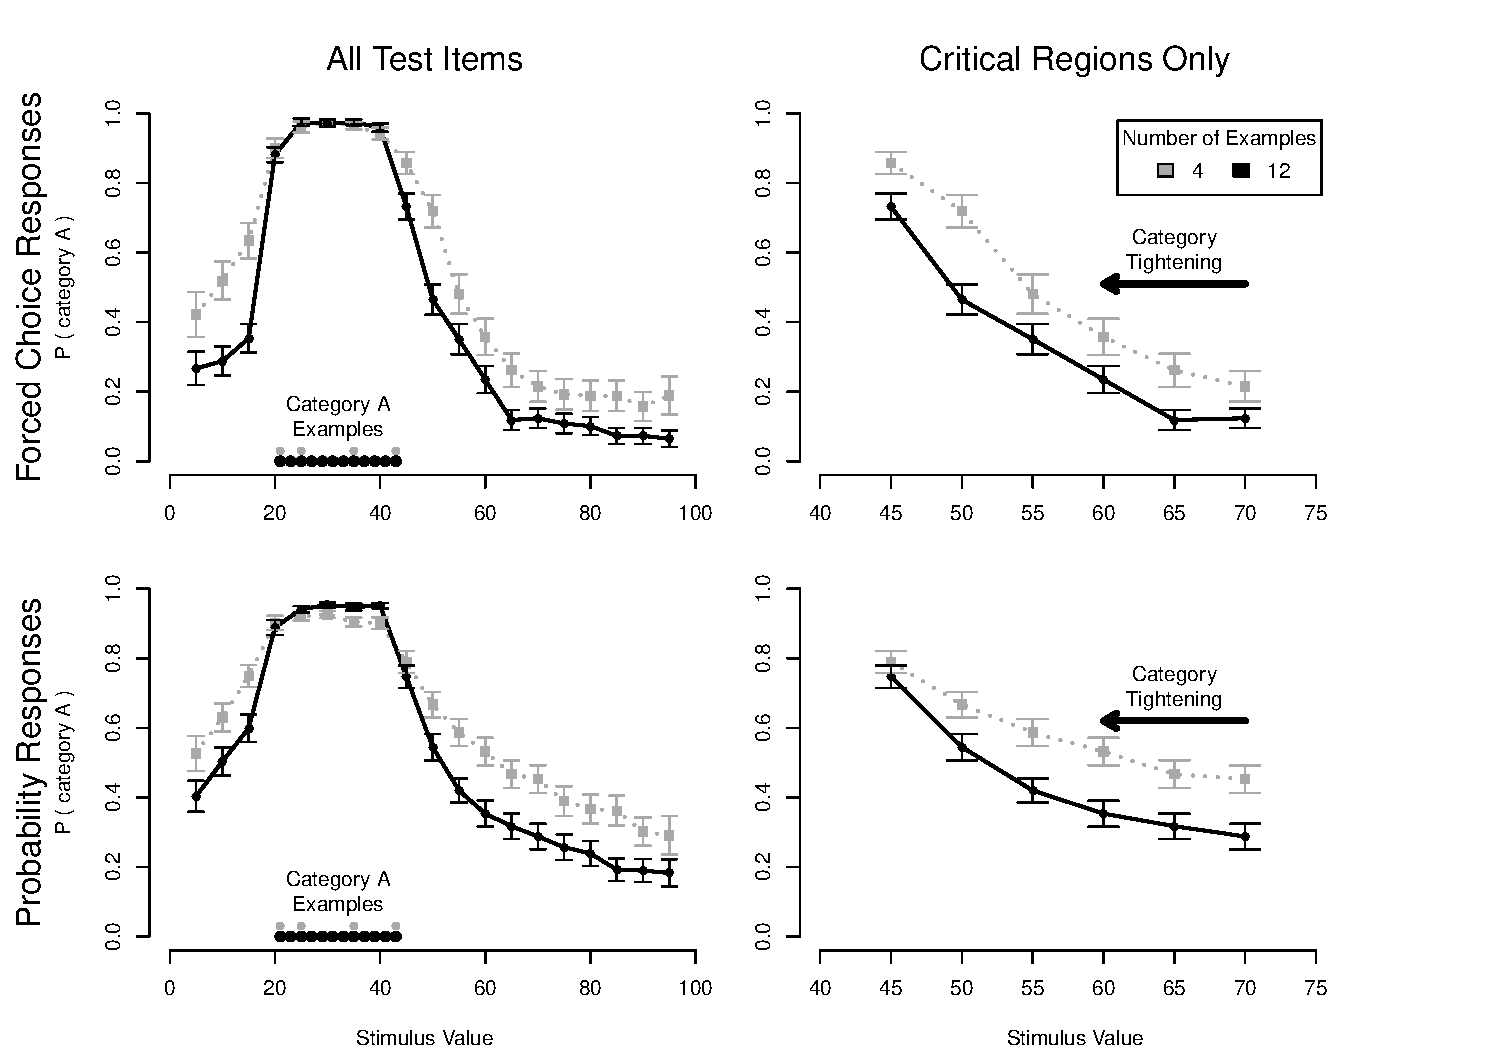
\includegraphics[width=5in]{figures/one_cat_results.pdf}
\end{tabular}
\end{center}
\caption{{\small  Human performance in the one-category experiment (Experiment 2). The top row shows the {\sc forced choice} condition: the proportion of answers selecting Category A in response to the question ``Do you think this example is in the category?'' for each possible stimulus value at test. The bottom row shows the {\sc probability} condition: the overall probability that the test item was rated as being in Category A. The graphs on the left show responses over the entire range of stimulus values; the ones on the right show responses in the critical range between the two categories from Experiment 1. Points along the gray line indicate responses after seeing {\sc four} exemplars; the black points indicate responses after {\sc twelve}. Participants who saw more observations in Category A {\it tightened} their responses for Category A. This is consistent with the predictions of the Bayesian model of generalization but not the GCM.}}
\label{fig:exp2results}
\end{figure}

The left column of Figure~\ref{fig:exp2results} shows participant responses during the test phase for all stimulus values, with the top row showing performance in the {\sc forced choice} condition and the bottom row showing performance in the {\sc probability} condition. Unlike in the previous experiment, the overall pattern for both response types shows a {\it decrease} in probability of assigning test stimuli to category A when more training examples are added.

We quantify these effects by comparing the same set of linear models as in Experiment 1, with responses in the {\sc forced choice} and {\sc probability} conditions analyzed separately.
Table~\ref{tab:expt2bayesfactors} shows the Bayes Factors for each of those three models; the model including only stimulus value serves as the baseline. It is evident from the table that the most preferred model in both the {\sc probability} and {\sc forced choice} conditions is the one that contains both stimulus value {\it and} the number of observations as predictors. This is evidence that people did in fact change their categorization probability when the category had more observations in it.

Examining the posterior estimates of the parameter values from the preferred model suggests that the eight extra training examples lead to a 13.3\% decrease in the probability of including the stimulus in the category
(95\% CI: 4.2\% to 22.7\%) in the {\sc forced choice} condition and a decrease of 12.4\% (95\% CI is 3.9\% to 21.0\%) in the {\sc probability} condition. By contrast with the previous experiment, this tightening is consistent with the predictions of the Bayesian model rather than the GCM.


\begin{table}[t]
  \centering
  \begin{tabular}{ccccc} % column spec
    \toprule
    Condition & Best Model & & Model Performance & \\
    \midrule
    & & Value & Value + Number & Interaction \\
    \midrule
    Forced Choice & Value + Number & $ 1 : 1 $ & $ \mathbf{12.9 : 1} $ & $ 1.5 : 1 $ \\
    Probability & Value + Number & $ 1 : 1 $ & $ \mathbf{14.0 : 1} $ & $ 10.3 : 1 $ \\
    \bottomrule
  \end{tabular}
  \caption{Comparison of how well three different regression models capture human performance in the two  conditions in Experiment 2. In both the {\sc forced choice} and {\sc probability} conditions, the preferred model contains both the stimulus value and number of observations as predictors. This suggests that, in keeping with the Bayesian model, people were less likely to classify an item as a member of the category if the category had more observations. See Table~\ref{tab:expt1bayesfactors} for model details.}
  \label{tab:expt2bayesfactors}
\end{table}

\subsection{Discussion}

The results in Experiment 2 are unambiguous. Regardless of whether people were asked to make forced choice decisions or to give probability judgments, increasing the sample size produced a tightening of the generalization gradients. As in Experiment 1, the estimated effect of the forced choice judgments appear to be more sensitive to the number of examples than the probability judgments. These results are consistent with \possessivecite{tenenbaum2001generalization} Bayesian analysis and inconsistent with the predictions from the GCM. Although the GCM provided the better account of the categorization problem in Experiment 1, the Bayesian model provided a much better account of the generalization problem in Experiment 2. This occurred even though the two tasks employed the same stimuli, the same instruction set, the same recruitment procedure, and the same response elicitation methods.

Experiments 1 and 2 examine the effect of increasing sample size on both generalization and categorization tasks.
Though the two tasks are conceptually closely related, the results indicate a clear difference.
Experiment 2 showed that additional exemplars caused people to tighten their inductive generalization when learning about a single category.
In contrast, Experiment 1 showed that such tightening was not evident in  people's categorization decisions, and indeed the reverse effect was observed in the {\textsc{Forced Choice}} condition.
If generalization and categorization are indeed closely related, then what might reasonably account for the differences observed?

The difference between the Bayesian model of generalization and Shepard's original model offers a possible explanation for these seemingly contradictory effects of increased sample size, in the form of the sampling assumption made by the learner.
When items from only a single category are seen, as in generalization experiments, a learner might be justified in assuming that the experiment is designed so that the only items that \textit{can} be shown are those that belong to the category.
This is equivalent to the strong sampling assumption from \citeA{tenenbaum2001generalization}, and predicts that the learner should produce generalization curves that tighten as sample size increases, as observed in Experiment 2 when items from only one category are present.

In a categorization task, where items from more than a single category are present, it is less clear how the learner should assume items are sampled.
One conservative possibility would be to assume that items are sampled in proportion to their base rate in the population, independent of the category label. This experimental design is not unusual in the categorization literature -- most often in the form of block randomized designs with equal base rates \cite<e.g.>{nosofsky1994comparing,lee2002extending,kruschke1993human,goldstone1994influences} -- and as such would not be unreasonable for a learner to assume in this task. From a Bayesian perspective, this sampling process is consistent with the {\it weak sampling} model \cite{shepard1987universalsim} where Equation~\ref{strongSampling} is replaced with a likelihood function that is independent of the size of the hypothesis:

\begin{equation}
\label{eq:weakSampling}
P(x_i | h) \propto \left\{ \begin{array}{lr} 1 & \mbox{ if } x_i \in h \\ 0 & \mbox{ otherwise} \end{array} \right.
\end{equation}


Under this account, the prediction about how generalization curves change depends on how category frequency information is integrated into the decision process (see Figure~\ref{fig:weakBayesianModelPredictions}).
If frequency information is not incorporated into the decision rule then generalization curves do not change at all as sample size increases (as in Equation~\ref{tgadapt1}).
If the decision rule includes priors based on category frequency (as in Equation~\ref{tgadapt2}), then generalization curves are predicted to expand as the relative frequency of the more frequent category increases.


\begin{figure}[t]
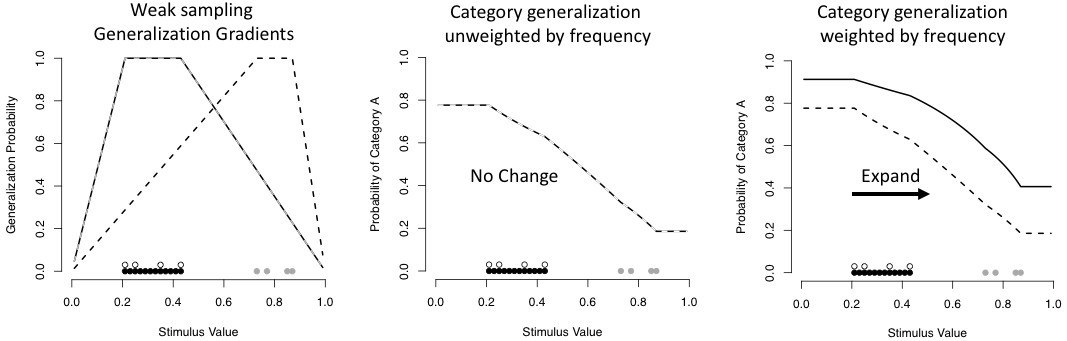
\includegraphics[width=1.0\textwidth]{figures/weakSamplingBayesianPredictions.png}
\vspace{-1mm}
\caption{%
Predictions from the Bayesian Generalization Model when assuming weak sampling (Equation~\ref{eq:weakSampling}). Left: Predicted generalization gradients where the 4-item and 12-item Category A curves exactly overlap (shown in black and dashed gray lines). Center: Category A generalization gradients using a decision rule without category frequency information (Equation~\ref{tgadapt1}). Increasing Category A frequency does not change the curve. Right: Category A generalization gradients using a decision rule that incorporates category frequency information (Equation~\ref{tgadapt2}). Increasing Category A frequency leads to category expansion.
}
\label{fig:weakBayesianModelPredictions}
\end{figure}


Thus, the contrasting results found in Experiments 1 and 2 may be explained by a shift in sampling assumptions based on the number of categories presented.  One way to test this account is by manipulating the beliefs learners have about why the frequency of the two categories are not equal.  If participants are dynamically adjusting their sampling assumptions based on the category structure, then it should be expected that they can adjust the degree to which category frequency influences generalization.  Experiment 3 tests this hypothesis using an extension of the two category design from Experiment 1.

\section{Experiment 3: Manipulating sampling assumptions}


This experiment replicates the \four\ exemplar condition of Experiment 1 as well as two variants of the original \twelve\ exemplar condition. In these two new conditions the set of training items is identical but the cover story for how items are sampled differs. The \random\ condition is designed to induce a weak sampling assumption by explaining that items are selected at random, independently from category membership.  In contrast, the \helpful\ condition is designed to induce a strong sampling assumption by encouraging the belief that items are chosen from a specific category by a helpful teacher. Experimentally manipulating sampling assumptions has been applied fruitfully in a number of inductive generalization tasks including word learning \cite{xu2007sensitivity}, property induction tasks \cite{ransom2016leaping,hayes2019diversity} and single category generalization tasks \cite{ransom2018representational, ransom2019samplingmemory}. The consistent finding in these studies is that experimentally manipulating the sampling assumption does have an effect on generalization. The question we consider in Experiment 3, then, is whether an analogous effect can be produced in a categorization task.

To our knowledge the only previous attempt to investigate this question in a multiple-category design is a study by \protect{\citeA{vong2013role}} who found some evidence that sampling assumptions can shape generalization from multiple categories. In this experiment we depart from that work in several ways. First, we use a more ``traditional'' learning task with stimuli explicitly displayed to participants, whereas \citeA{vong2013role} presented stimuli schematically as a distribution of points along a single dimension, as in \citeA{navarro2012sampling}. Second, the sample size manipulation in \citeA{vong2013role} increased the number of items in both categories rather than one of two as in our Experiment 2. Third, in their two-category study participants were only queried about ``category A'', a framing which could plausibly have caused people to focus more on one category, rather than asking the more neutral classification question (i.e., ``A or B'') used in the previous experiments.  With these considerations in mind, our Experiment 3 revisits this question, using a procedure similar to Experiments 1 and 2.

\begin{figure}[t]
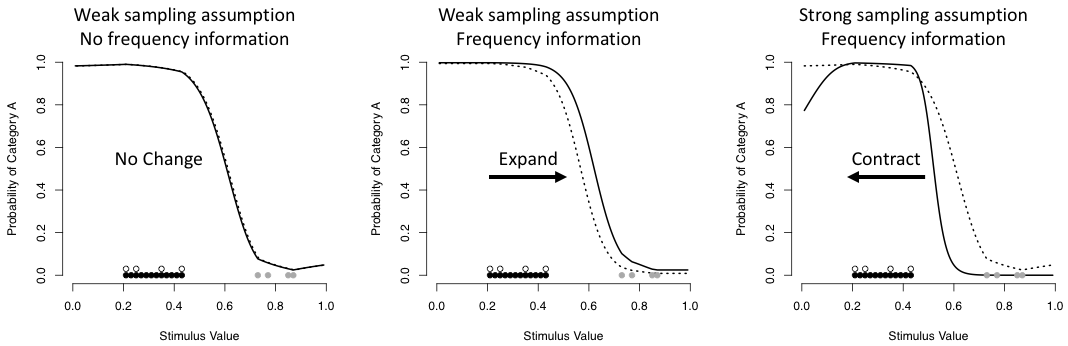
\includegraphics[width=1.0\textwidth]{figures/exp3-predictions.png}
\vspace{-1mm}
\caption{%
Three possible patterns of results in Experiment 3.
The left panel is produced by assuming weak sampling and no frequency information in the decision rule.
The middle panel is produced by a model that assumes weak sampling but includes frequency information when making a decision.
The right panel is produced by a model that assumes strong sampling which inherently includes frequency information.
}
\label{fig:exp3-predictions}
\end{figure}

%As outlined above, if the two category categorization task induces a weak sampling assumption then manipulating the perceived source of the category frequency difference makes two predictions about the expected difference in generalization between conditions.

Our goal in this experiment is to provide people with a plausible explanation as to \textit{why} they are seeing more examples of one category than another in the two twelve exemplar conditions. By purporting to select items at random, the \random\ condition is designed to promote the belief that the different sample sizes are reflective of the true category base rates. By contrast, in the \helpful\ condition people are led to believe that the number of exemplars provided is simply a constraint imposed on the selections made by the helpful teacher and therefore not reflective of the true base rates.

By comparing performance across these three conditions, we are able examine the effect of additional exemplars on generalization and to test whether the nature of the effect changes depending on the learner's assumptions. In making such comparisons, there are three different patterns of results that we might reasonably expect, as illustrated in Figure~\ref{fig:exp3-predictions}. If a two category categorization task, by its nature, induces a weak sampling assumption (regardless of our cover story), we predict the following two effects.  First, people who observe twelve randomly sampled category A exemplars should attribute the difference in sampling frequency to a genuine difference in category base rates. As a consequence, these people should widen their generalizations away from category A when compared with people who see only four category A exemplars (middle panel).  Second, people who believe that the eight additional exemplars were sampled from the category should show no change in their generalizations toward category A relative to people in the \four\ condition (left panel).  If, however, the \helpful\ sampling cover story is sufficient to lead people to believe that each item was strongly sampled from its respective category, then their generalizations should tighten toward category A relative to people who only saw four category A exemplars (right panel).

\subsection{Method}

\subsubsection{Participants}

We recruited 364 participants for this experiment via Amazon Mechanical Turk. Of
these, 20 people were excluded from participation, having taken part in either
of the previous experiments. No results were collected from 31 people who failed
to complete the experiment. A further 15 people were excluded from further
analysis for failing to reach the predefined accuracy threshold used in Experiment 1. Data from the remaining 298 participants were included in all subsequent analyses. Participants ranged in age from 18 to 68 (median age: 32), 39\% were female, and 98\% of participants were from the USA. Participants were paid \$USD 1.25 for taking part in the 7 minute experiment.

\subsubsection{Design}

People were allocated at random to one of three conditions.
People in the \neutral\ condition ($N=96$) were shown four exemplars from
category B and four from category A, with no explanation offered for how these
examples were chosen.
%
Likewise, participants in the \helpful\ condition ($N=99$) saw four
exemplars from each category for which no explanation was offered. However, in
addition they saw a further eight exemplars from category A which, they
were told, had been selected from the category by a helpful teacher.
%
In the \random\ condition ($N=103$), people were told that 16 examples had been
chosen for them at random. The ``random'' selection always consisted of the four
category B exemplars, and twelve exemplars from category A.

\subsubsection{Stimuli}

The overall design of the study was based on Experiment 1.
%
The stimuli were identical in appearance
to those in the previous study (albeit that the images were allowed to
scale to fit within the user's browser window in a manner that preserved the
original aspect ratio).
%
However, we restricted the presentation of the stimuli so that the black line
within the stimuli varied only by position, with category A exemplars always
represented by a line toward the left (the details of how the black line varied
having made no material difference in the previous study).
%
The same stimulus values were also used, as well as the same method of
determining the subset of category A exemplars seen by participants in the
\neutral\ condition.

\subsubsection{Procedure}

The experiment followed the same basic procedure as Experiment 1, the main
difference being the initial explanation of the experiment given prior to the
training phase. Participants in all conditions were told that the purpose of the
experiment was to see how well they could judge between two categories of
similar looking objects. Participants were then informed how examples would be
selected. This explanation differed across the three conditions. People in the
\neutral\ condition were told simply:
%
\begin{quote}
  We'll start by showing a few examples of each category, taken from our catalogues.
\end{quote}
%
\noindent at which point the four category B and four category A exemplars were
displayed on-screen. Participants in the \helpful\ condition were given
this same introduction. However, after the initial exemplars were displayed,
they were informed:
%
\begin{quote}
{\bf The computer has assigned you to experiment group {\tt <<{\bf K8}>>}}, so we're
going to help you by showing you an additional {\tt <<8>> <<Wuggams>>} {\bf chosen by a helpful teacher} from our Wuggam catalogue.
\end{quote}
%
\noindent People in the \random\ condition were told the following:
%
\begin{quote}
{\bf The computer has assigned you to experiment group {\tt <<{\bf J16}>>}}, so
we'll start by {\bf selecting {\tt <<{\bf 16}>>} objects at random} from our catalogue. We'll classify the objects on-screen for you so that you have some examples to work with.
\end{quote}
%
All subsequent instructions were identical across conditions.

As with Experiment 1 \& 2, the training stimuli remained on-screen during the
testing phase, and were annotated with a reminder of how the stimuli were
chosen. Based on the assumption that forced choice decisions are more sensitive to
changes than probability judgments, the response measure was limited to
{\textsc{Forced Choice}} in all three conditions. Otherwise, the conduct of the
test phase followed the procedure adopted in Experiment 1.

\subsection{Results}

\begin{figure}[htbp]
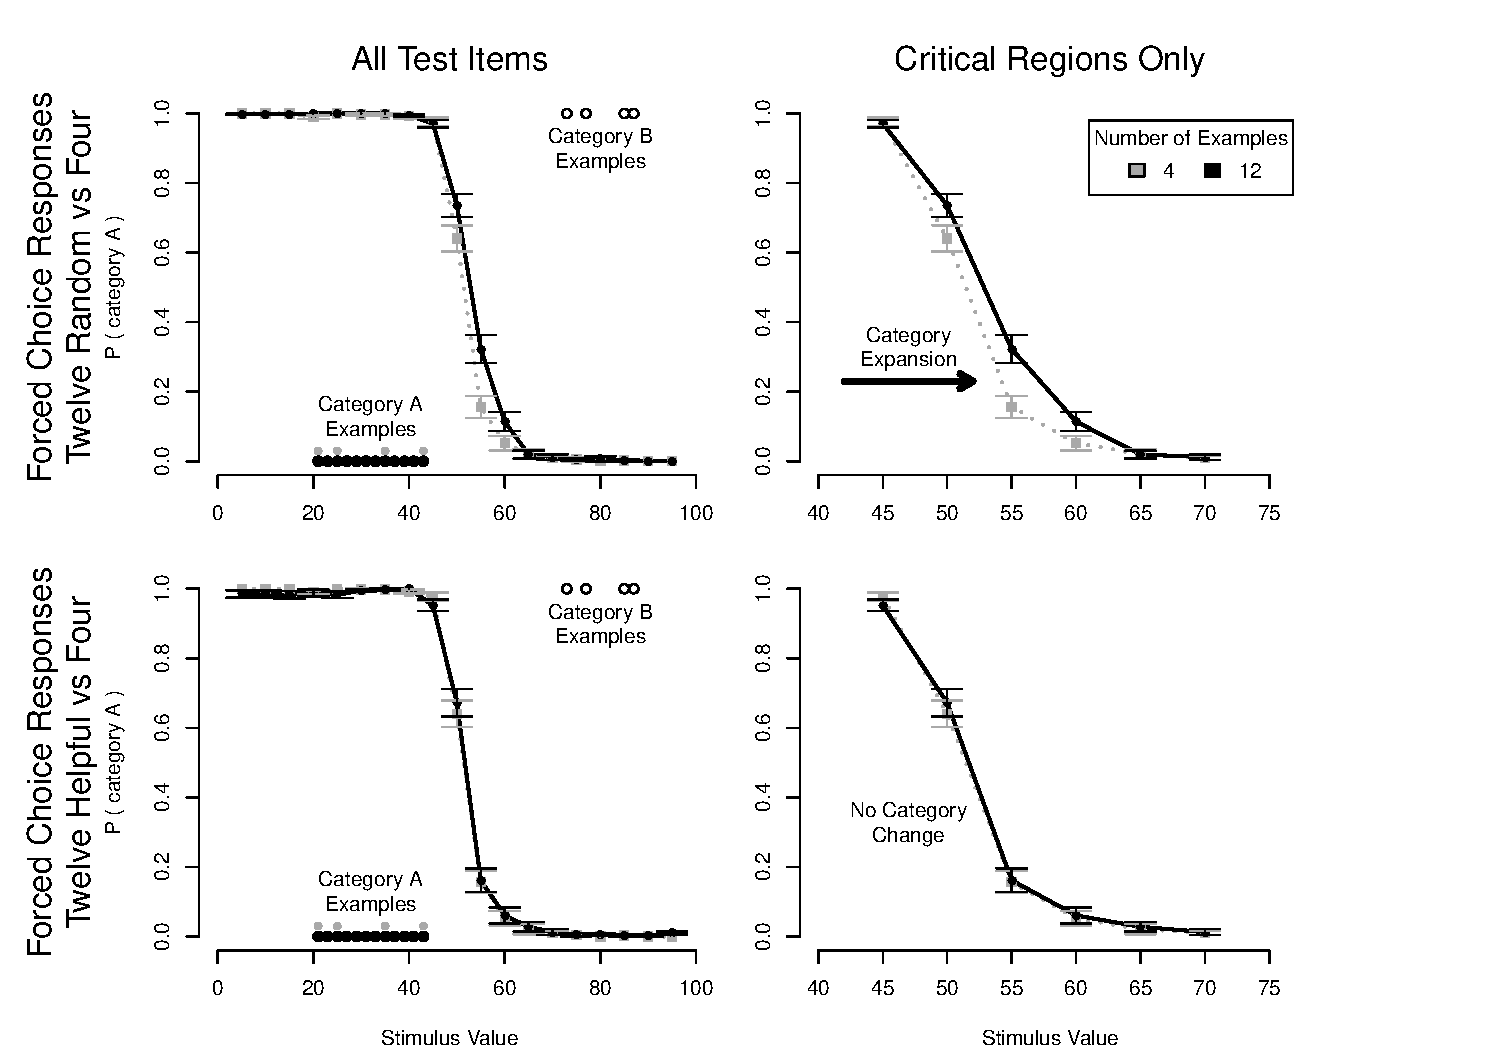
\includegraphics[width=1.0\textwidth]{figures/two_cat_sampling_results.pdf}
\vspace{-1mm}
\caption{%
Human performance in the two category experiment with sampling assumption
manipulation (Experiment 3).
%
The graphs show the proportion of responses
selecting category A in response to the question: ``Which category do you think
this example belongs in?'' for each possible stimulus value at test.
%
The graphs on the left show responses over the entire range of stimulus values;
those on the right show responses for stimuli in the range between the two
categories.
%
Each row contrasts the performance of people who saw four category A exemplars
(shown in gray) with one of the groups that saw
twelve (shown in black): \random\ in the top row, and \helpful\ in the bottom row.
%
The effect of additional exemplars differs depending on
condition. People who are told that all exemplars are
selected at random from a collection of objects are more likely to assign items to
category A. In contrast, those who are told that an additional eight exemplars had been chosen by a
helpful teacher, exhibited near identical responses to people who see only four
exemplars.
}
\label{fig:exp3-results}
\end{figure}

The overall pattern of responses is consistent across all conditions, with
people more likely to indicate that lower stimulus values were in category A,
while higher values were in category B (\Cref{fig:exp3-results}). Importantly, the pattern of responses is broadly consistent with that of Experiment 1 (\Cref{fig:exp1results}).
%
% Thus, we may use the results of the current study to examine if the expansionary effect of additional exemplars observed in Experiment 1 was due to the assumptions on the part of the learner that the two category nature of the experiment induced.

% KR: Strictly speaking I think it may be misleading to talk about the different explanation for the "additional" observations, since in the Random condition we explained all 16 exemplars.
% \cref{fig:exp3-results} shows the effect of additional observations on people's responses.
% Did the difference between the explanation of the additional observations in the \random\ and \helpful\ conditions?
% We examine this by first comparing both conditions to the \neutral\ condition .
The \random\ and \helpful\ conditions have different cover stories to explain how the training items are sampled. Did people generalize differently on the basis of the explanation they receive?
We examine this by comparing both of these conditions to the \neutral\ condition.
People in the \random\ condition (top row of Figure~\ref{fig:exp3-results}, responses shown in black) are more likely to classify test stimuli as belonging to category A than people in the \neutral\ condition (response shown in gray).
%
In contrast, people in the \helpful\
condition (bottom row), who are told that the eight additional exemplars had been selected
from the category by a helpful teacher, show a similar pattern of response to people in the \neutral\ condition.

In order to quantify these effects, three contrasts were created based on subsets of the data.
For each contrast, we calculate the posterior odds for
the three linear models defined in Experiment 1.
To determine which of the three models best captures the data for each contrast, Bayes factors for each model are constructed relative to the \valueonly\ model.

First, we compare performance in the \random\ and \helpful\ conditions to determine if the instruction manipulation changes how people processed the observations (top row of Table~\ref{tbl:exp3:bf1}).
% KR: The wording "includes a difference between the conditions"
% sounds a bit unusual. I've had a go at condensing. Feel free
% to reject of course.
% This comparison favors the interaction model, which includes a difference between the \random\ and \helpful\ conditions.
% This indicates the two conditions with two items produce different generalizations but not how they differ from the \four\ observation condition.
This comparison favors the interaction model, indicating that the two conditions that differ only in their cover story produce different generalizations.

To determine how the change in generalization due to more observations is impacted by the instruction manipulation, both twelve-item conditions are compared to the \four\ observation condition (middle and bottom rows of Table~\ref{tbl:exp3:bf1}).
The results mirror the qualitative patterns in Figure~\ref{fig:exp3-results} and show markedly different results for the two contrasts.
The contrast between the \neutral\ and the \random\ conditions is best captured by the \interaction\ model that indicates a difference between conditions.
% both a difference between conditions as well as an interaction with stimulus value.
This is not the case for the contrast between the \neutral\ and \helpful\ conditions, which is best captured by the \valueonly\ model, suggesting that with the helpful instruction manipulation there is no effect of additional category items.

% KR: Updated on Feb 3, 2019.
% KR: Output of Bayes Factor analysis for Neutral vs Random
% Bayes factor analysis
% --------------
% [1] exemplar + uid                                  : 1        ±0%
% [2] exemplar + condition + uid                      : 2.532111 ±0.99%
% [3] exemplar + condition + exemplar:condition + uid : 190.6518 ±0.52%
%
% Against denominator:
%   count ~ exemplar + uid

% KR: Output of Bayes Factor analysis for Neutral vs Helpful
% Bayes factor type: BFlinearModel, JZS
%
% Bayes factor analysis
% --------------
% [1] exemplar + uid                                  : 1            ±0%
% [2] exemplar + condition + uid                      : 0.1054419    ±0.94%
% [3] exemplar + condition + exemplar:condition + uid : 0.0002769069 ±1.05%
%
% Against denominator:
%   count ~ exemplar + uid
% ---
% Bayes factor type: BFlinearModel, JZS
%
% Helpful 12 vs Random 12
% Bayes factor analysis
% --------------
% [1] exemplar + uid                                  : 1        ±0%
% [2] exemplar + condition + uid                      : 1.284412 ±0.49%
% [3] exemplar + condition + exemplar:condition + uid : 7.200172 ±3.53%
%
% Against denominator:
%  count ~ exemplar + uid
% ---
% Bayes factor type: BFlinearModel, JZS

\begin{table}[tbp]
\hspace{-5mm}
\small
\begin{tabular}{lcrrr}
\toprule
 & & \multicolumn{3}{c}{Bayes Factor (relative to \valueonly)} \\
\cmidrule{3-5}
Contrast & Best Model & \valueonly & \textsc{Value + Condition} & \interaction \\
\midrule
\bothtwelve\ & \interaction & $1 : 1$ & $1.3 : 1$ & $\mathbf{7.2 : 1}$\\
\neutral\ vs. \random\ & \interaction & $1 : 1$ & $2.5 : 1$ & $\mathbf{190 : 1}$ \\
\neutral\ vs. \helpful\ & \valueonly & $\mathbf{1 : 1}$ & $0.11 : 1$ & $2.8 \times 10^{-4} :1$\\
\bottomrule
\end{tabular}
\caption{%
Comparison of how well three different linear regression models capture the results from subsets of the two category experiment with sampling assumption manipulation (Experiment 3).
%Each subset of the full data represents a different contrast of interest.
%
Top row: Contrasting the results from the \helpful\ and \random\ conditions shows that the \interaction\ model, which includes both
stimulus value and the condition (random instructions or helpful instructions), as well as an interaction term, best captures the data.
%
Middle row: Similarly, the contrast between the \neutral\ and
\random\ conditions is also best explained by the \interaction\ model which includes differences between the \four\ and \random\ conditions.
%
Bottom row: In contrast, analysis of data from the \neutral\ and
\helpful\ conditions shows that the \valueonly\ model, without any difference between the the \four\ and \helpful\ conditions, best captures the data.
%
Bayes factors are expressed as odds ratios against the \valueonly\ model reported to two significant figures.
% Taken together these results suggest that extra observations in category A are not sufficient to drive expansion of the category boundary. Additional assumptions, such as the representativeness of observed category frequencies, may also be required in order to drive expansion.
}
\label{tbl:exp3:bf1}
\end{table}





\subsection{Discussion}

The results from Experiment 3 indicate a difference in generalization due to a cover story manipulation of how items were sampled.
People who were told the items come from a helpful teacher did not show any category expansion when seeing additional items, but people who were given no explanation did show category expansion.

%that people who are shown 12 items category A items and told they were selected by a helpful teacher show
% Experiment 3 shows a clear difference between the generalization curves produced by the random and helpful cover stories.

While these patterns are consistent with the predictions of the two-category GCM (Figure~\ref{fig:gcmExample}), a compelling account of why the cover story difference between the \random\ and \helpful\ conditions changes generalization behavior is lacking.
Furthermore, the lack of change in the category generalizations as a function of category frequency in the \helpful\ condition provides a demonstration that relative frequency alone does not ensure category expansion. Instead, the effect of category frequency seems to be moderated by assumptions about how items are sampled.

These results are more challenging for the two-category Bayesian Generalization model that assumes training items are strongly sampled (Figure~\ref{fig:bayesExample2}).
Indeed, the predictions of this model do not match the observed pattern of results.
However, the predictions of the weak sampling versions of this model do (left and center panels of Figure~\ref{fig:weakBayesianModelPredictions}).
%AP: this said center and right, I think you meant centre and left
% DH: yep, I got that wrong or the figure order changed in revisions.
Specifically, generalization in the \helpful\ condition, which provides an explanation of the frequency difference that is not connected to base rates, matches the generalization pattern of the weak sampling Bayesian generalization model that does not incorporate base rate information into the decision rule (left panel). The \random\ condition, which does not provide an
% KR: The use of "alternative explanaion" could be made clearer - alternative to what?
explanation of the difference in category frequency, matches the predicted pattern of the weak-sampling Bayesian Generalization model that incorporates base rate information into the decision rule (middle panel).\footnote{One possibility is that since the presentation of the test stimuli was similar in all conditions and appeared superficially more similar to weak sampling, the strong sampling manipulation may not have been strong enough to overcome this. This is an interesting avenue for future work, but for now we note that because the test procedure was the same in all conditions it cannot be responsible for the key finding of Experiment 3, which was the change in behavior between the {\sc Twelve Random} and {\sc Twelve Helpful} conditions.}

Rather than supporting the strong sampling Bayesian Generalization model in a categorization task, these results are more consistent with a shift in the Bayesian Generalization model to an assumption of weak sampling in the presence of items from two categories.
However, much like the GCM, the Bayesian Generalization framework does not predict why the shift in sampling assumptions occurs. This issue is addressed in the next section.

% Furthermore, these patterns, when matched to the of the extended Bayesian generalization model in which category frequency contributes to inference about sampling assumptions.

% Let us first consider the \random\ condition, which was designed to persuade
% participants that items were sampled from a set of objects, and in such a way
% that relative differences in the number of items observed in each category were
% reflective of true differences in base rates.
% This condition is very similar to the non-cover story in Experiment 1 and, as before, the category A generalization curve expands as the frequency increases.
% This pattern is inconsistent with the Bayesian generalization model that assumes strong sampling, but is consistent with the GCM as well as the modified Bayesian generalization model that assumes weak sampling of training items and incorporates category frequency information into the decision rule (illustrated in the right panel of Figure~\ref{fig:weakBayesianModelPredictions}).

% The \helpful\ condition in contrast, was designed to persuade participants that the items were not selected randomly and therefore not in proportion to the base rate of the categories.
% Interestingly, this produced generalization curves that did not change relative to the \four\ condition.
% % This pattern of results suggests that these instructions did not result in participants assuming that the items were sampled only from category A, which is strong sampling and thus would have predicted tightening of the generalization curve.
% As in the \random\ condition, this pattern is consistent with the assumptions of the weak-sampling Bayesian model and not the strong-sampling model, but only if the decision rule does not include information about category frequency (illustrated in the center panel of Figure~\ref{fig:weakBayesianModelPredictions}).
% %Instead, the instructions resulted in participants assuming weak sampling and a decision rule that does not include information about category frequency, resulting in no change to the generalization curves.


%%%%%%%%%%%%%%




\section{General Discussion}

Taken together, the results from Experiments 1 and 2 paint a clear picture: the effect of increasing sample size is qualitatively different in categorization tasks and generalization tasks. In an inductive generalization problem, the learner is presented with positive examples that belong to a single category, and asked to determine whether novel items also belong to this category. In the generalization context, the Bayesian generalization model developed by \citeA{tenenbaum2001generalization} makes a clear prediction that is replicated here:  increasing the sample size without expanding the region of psychological space spanned by the exemplars should cause people's generalizations to tighten. This is precisely what Experiment 2 found.

In the categorization context, the opposite pattern holds. The exemplar model predicts that if we increase the sample size for one category without changing the region of psychological space that it covers, then the effect should be very small and in the opposite direction: a {\it category frequency} effect should apply and as a consequence the categorization boundary should move {\it away} from the category. This is precisely what Experiment 1 found.

In one sense the results should be unsurprising: as a categorization model, the GCM outperforms the Bayesian model on categorization problems; and as a generalization model the Bayesian model outperforms the GCM on generalization tasks. However, unless one is prepared to give up on the notion that categorization and generalization are related inductive problems, this is not a terribly satisfying answer.

Experiment 3 attempted to test one possible explanation for the generalization differences between categorization and generalization: that learners in the two tasks make different assumptions about how the items are sampled. Without a method that could explicitly measure sampling assumptions, we turn instead to directly manipulating sampling assumptions via the cover story. The results indicate that participants not given a justification for the difference in category frequency show expansion of the more frequent category, while participants given a justification beyond true category frequency show no such expansion.

\subsection{Addressing the inconsistency: the Bayesian generalization model}

From the Bayesian perspective, a natural resolution to this inconsistency is to argue that participants bring different inductive biases to one-category generalization and multi-category categorization tasks. We might expect that in a generalization task, the {\it mere fact} that the experiment presents positive examples from a single category suggests that items are generated by sampling from items within the category. If this strong sampling assumption properly describes the learner's theory of the experimental task, then the size principle holds and as a consequence we should expect generalization gradients to narrow as more data are received. When presented with a single category to learn about, this seems to be exactly what people assume is generating the items.

In a categorization task, it is not at all clear what sampling model should be appropriate. %that the participant should assume a strong sampling model.
% AP: I changed this because it seems to be contradicting the rest of the paragraph, unless I"m missing something.
The Bayesian categorization model outlined earlier in the paper is based on the assumption that the experiment generates stimuli via a two stage procedure. On any given trial the experimenter first selects a category (with probability given by the category frequencies); then having chosen a category, the experimenter chooses an exemplar {\it from} that category. This sampling procedure is the natural analog of the strong sampling model, as applied to a categorization task. It is not an inherently unreasonable assumption for a participant to make. Many real world categorization problems have a similar flavor, in which the categories are selected first, and then exemplars are sampled from those categories.
The set of players competing in a soccer game come from such a sampling procedure: the two teams (categories) are first selected by the league and then players (item exemplars) from those teams define the set of players.
% When watching a football game, for instance, the fixture selects the categories (teams) and then the exemplars (players) that one observes are drawn from those categories.

As reasonable as this sounds, it is by no means the only assumption that people might make about how a categorization task is designed. In a weak sampling model (as per \possessivecite{shepard1987universalsim} original description), the causal ordering is reversed: the world (or the experimenter) is assumed to have a fixed set of exemplars to choose from, and those exemplars are sampled independently of the category to which they belong. Again, there are many real world scenarios that have this flavor. For example, when trying to guess the colors of vehicles, it seems natural to think that the world selects directly from the set of cars (item exemplars) without considering the color category to which they belong.

Critically, under a weak sampling assumption, the size principle does not hold and thus generalizations should not tighten \cite{tenenbaum2001generalization,tenenbaum1999bayesian}. If people adopt this kind of sampling model in a categorization experiment -- and assume that the experimenter chooses directly from the set of exemplars -- then the corresponding Bayesian model does not predict a tightening effect. Specifically, such a model would predict little to no effect of sample size, or an expansion due to a category frequency effect in the prior probability of the category labels that change with additional exemplars.
What becomes less clear is how weak sampling alone (absent category frequency information) can account for the difference between the random and helpful cover stories in Experiment 3.

Our point is not that the Bayesian model is incapable of capturing the effects seen in these experiments. Rather, our point is that it appears to account for one (tightening) quite naturally while the other (expansion) is less well theoretically motivated and more {\it post hoc}. Why should people prefer one sampling scheme over another in these different situations? Why, when shown a set of Daxes, do people appear to assume that the experimenter deliberately selected items from the {\it target category}, but when shown Daxes and Wugs they appear to assume that the items were selected from {\it the set of objects}? Since this difference arose even though the all other aspects of Experiment 1 and 2 were the same, the answer is not due to stimulus differences or response methods. Either the learners made different assumptions in Experiments 1 and 2 about how many categories {\it existed}, or they made different assumptions about how they were {\it sampled}. In this context, these assumptions are impossible to tell apart and make the same prediction about what stimuli people expect to be presented with. A Bayesian model of how people perform both generalization and categorization must allow the learner to infer information not only about the hypotheses of the category structure, but also about how items are sampled. However, this dynamic updating of the likelihood function based on the items sampled is also impacted by the cover story, as shown in Experiment 3.
%AP: I modified this paragraph to address the comments from the editor and the reviewer. The old text is below.

%, or cover story.\footnote{Strictly speaking, the cover stories do differ between Experiments 1 and 2, to the extent that the instructions describe slightly different tasks, and this difference in instructions may affect people's beliefs about sampling \protect\cite<e.g.,>{ransom2016leaping}. In this context, we simply mean that the cover stories in Experiments 1 and 2 were matched in every respect \textit{other} than those required to describe the differences between tasks.} Instead, a Bayesian model of how people perform both generalization and categorization must allow the learner to infer information not only about the hypotheses of the category structure, but also about how items are sampled. However, this dynamic updating of the likelihood function based on the items sampled is also impacted by the cover story, as shown in Experiment 3.

%We now turn to a consideration of the GCM. Can it be modified to predict both effects, and are those modifications more theoretically motivated and less post hoc than the modifications to the Bayesian model?

\subsection{Addressing the inconsistency: the exemplar-based categorization model}

The similarity-based exemplar framework offered by the GCM correctly predicts what happens in categorization tasks, but the straightforward adaptation of the model we implemented makes exactly the wrong prediction in the generalization problem. According to that model, as shown in Figure~\ref{fig:gcmExample2}, the response strength for the category increases but the criterion against which it is compared does not, producing the expansion effect.

We can produce a different prediction by proposing an alternative decision criterion. Suppose people automatically adjust the threshold to compensate for the rise in response strength for the target category. If, as in \citeA{nosofsky2011short} where the threshold depends on list length in a recognition memory task, the threshold ($\phi$) for accepting a new item increases as a linear function ($m$) of category frequency ($N$) then Equation~\ref{gcm4} would be replaced with

\begin{equation}
\label{gcm5}
P(y \in c) = \frac{\eta(y,c)}{\eta(y,c) + mN}
\end{equation}

\noindent
and the predictions of the model now become rather different. As Figure~\ref{fig:gcmExample3} illustrates, if the multiplicative factor for the relationship between threshold and sample size is one, the GCM now predicts a null effect of sample size in Experiment 2. Furthermore, by also changing the stimulus generalization parameter $\lambda$ and the slope $m$, this version of the GCM {\it can} produce the qualitative tightening of generalization curves observed in the data.

%By extension, of course, it is clear that the GCM {\it can} accommodate the qualitative tightening of generalization curves in the observed data perfectly well, simply by assuming that the scaling factor $m$ is larger than one.

Other theoretical approaches to this issue are also possible. For instance, previous work examining how response bias and category variability are related \cite{cohen2001category} offers one possible answer. One might imagine that response biases are adjusted strategically as a consequence of the assumed sampling process, which would account for the results in Experiment 3. Another possible theory would connect the stimulus generalization parameter $\lambda$ to assumptions about sampling, as previous work has shown excellent fits to data when this parameter varies as a function of memory strength due to serial position in memory tasks \cite{donkin2012power,nosofsky2011short}.
Formalizing \textit{post-hoc} relationships about how these parameters should change as a function of sampling assumptions and category frequency is beyond the scope of this work, but it clearly requires integrating information about how learners reason about both sampling and frequency.

\begin{figure}[t]
\begin{center}
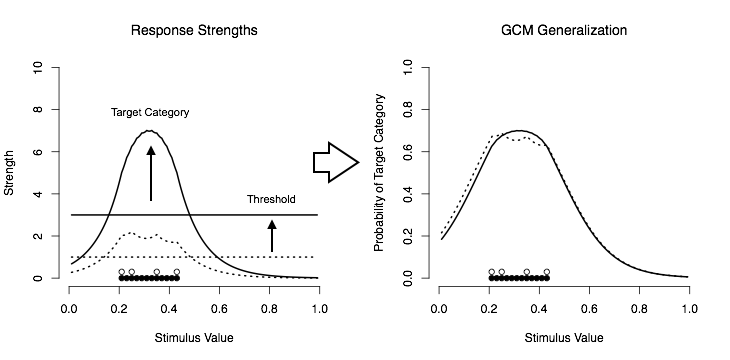
\includegraphics[scale=.5]{figures/modifiedGCM.png}
\caption{Modified generalization behavior in the GCM when the threshold scales linearly ($m = 1$) with sample size. The model now predicts that sample size should have no effect on people's willingness to endorse the category.}
\label{fig:gcmExample3}
\end{center}
\end{figure}




\subsection{Sampling assumptions and category frequency}

What then is the appropriate model of how learners incorporate information about the number of categories, the frequency of those categories, and their assumptions about how categories and items are sampled? The results from these experiments suggest the relationship involves two moving parts. First, learners appear to shift from category frequency dependent reasoning in a one-category generalization context to a frequency independent reasoning in a two-category categorization context. Second, the role of category frequency information in categorization is flexible and depends on the assumptions the learner makes about how items are sampled.
Though this poses a challenge to existing theories of both categorization and generalization, treating categorization and generalization as fundamentally different tasks fails to capture the flexible nature of human cognition as it adapts and shifts beliefs as more information becomes available.

\section{Acknowledgments}

DJN received salary support from ARC grant FT110100431 and AFP from ARC grant DE120102378 . Research costs and salary support for ATH were funded through ARC grants DP110104949 and DP150103280. KR was supported by an Australian Government Research Training Program Scholarship.
Preliminary versions of this work were presented at the 48th and 50th Annual Meeting of the Society of Mathematical Psychology.
We would like to thank Robert Nosofsky and two anonymous reviewers for their helpful comments on a previous version of this article.


\nocite{*}
\bibliography{citations,bayes_gen_papers,categorization_frequency_papers,gamma_discussion_citations}


\section*{Appendix: Bayesian multi-category generalization}

To derive a multiple-category version of the Bayesian generalization model, we adopt a formalism very similar to the \citeA{tenenbaum2001generalization} model, which in turn builds on the formal approach developed by \citeA{shepard1987universalsim}. Let $\bm{x}=(x_1,\ldots,x_N)$ denote a set of $N$ items that lie in a bounded unidimensional space, which we assume to be $x_i \in [0,1]$ without loss of generality. These items are sampled from one of $K$ categories, where we let $\bm{c}=(c_1,\ldots,c_N)$ denote the category from which each exemplar is drawn, $c_i \in (1,\ldots,K)$. For simplicity we assume that each item belongs to exactly one category, but the extension of the categories along the stimulus dimension can overlap.

Given this set up, the learning problem is formalized as follows. On any given trial the category label $c_i$ is chosen (by the experiment) at random, where the probability $P(c_i = k)$ of selecting the $k$-th category is denoted $\theta_k$. This probability is unknown a priori to the Bayesian learner, and for simplicity we assume the learner places a uniform prior $P(\bm\theta) \propto 1$ over these probabilities. Having chosen the category $c_i=k$, the experiment (or experimenter) next selects the exemplar $x_i$ to present to the learner. The $k$-th category is associated with a particular ``consequential region'' of the stimulus space, $h_k$, and we assume that the specific exemplar is selected uniformly at random from that region. In \possessivecite{tenenbaum2001generalization} terminology this is a {\it strong sampling} model:
$$
P(x_i|c_i=k,h_k) = \left\{ \begin{array}{cl} 1/|h_k| & \mbox{ if } x_i \in h_k \\ 0 & \mbox{ otherwise} \end{array} \right.
$$
where $|h_k|$ denotes the {\it size} of the consequential region. \citeA{shepard1987universalsim} adopts the assumption that every category occupies a connected region within the stimulus space, which for a unidimensional space $\mathcal{X}$ corresponds to an interval $[l_k, u_k]$. Shepard's ``connected region'' assumption has been adopted in a number of other papers \cite<e.g.,>{navarro2012sampling} but has been relaxed in other contexts \cite<e.g.,>{tenenbaum2001generalization,navarro2006natural}. Our application is simple enough that Shepard's original assumption will suffice, and under this assumption the size of category $k$ is simply the length of the corresponding interval $|h_k| = u_k - l_k$. The structure of the model is illustrated in Figure~\ref{pic2}.

\begin{figure}[t]
\centering
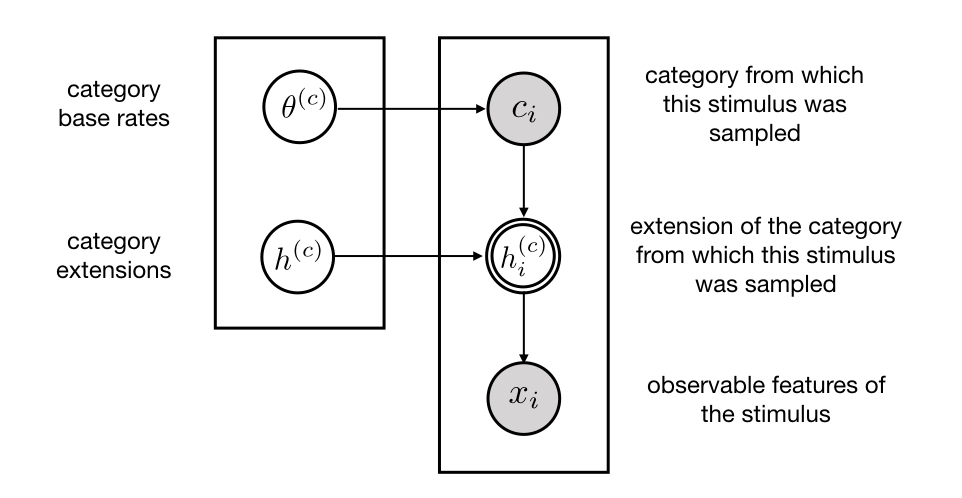
\includegraphics[width=.9\textwidth]{figures/twocatgraphicalmodel.jpg}
\caption{Probabilistic model for the training data.}
\label{pic2}
\end{figure}

\subsection*{Using information about category extensions and base rates}

We let $\bm{h}=(h_1,\ldots,h_K)$ denote the true consequential regions for each of the $K$ categories, and assume that the learner places independent and identical priors over each of these regions $P(\bm{h})=\prod_{k=1}^K P(h_k)$. Given the training exemplars $\bm{x}=(x_1,\ldots,x_N)$ and their corresponding labels $\bm{c}=(c_1,\ldots,c_N)$, a Bayesian reasoner learns about the category extensions $\bm{h}$ and base rates $\bm{\theta}$ as follows
\begin{eqnarray*}
P(\bm{h},\bm{\theta} | \bm{x}, \bm{c})
&\propto& P(\bm{x}, \bm{c} | \bm{h},\bm{\theta}) P(\bm{h},\bm{\theta}) \\
&=& P(\bm{x} | \bm{c}, \bm{h})  \times P(\bm{h}) \times  P(\bm{c} | \bm{\theta}) P(\bm{\theta}) \\
&=&  \prod_{i=1}^N P(x_i | c_i, h_{c_i})  \times \prod_{k=1}^K P(h_k)  \times P(\bm{c} | \bm{\theta}) P(\bm{\theta}) \\
&=&   \prod_{k=1}^K \left( P(h_k) \prod_{i|c_i=k} P(x_i | c_i=k, h_k) \right)  \times  P(\bm{c} | \bm{\theta}) P(\bm{\theta}) \\
& \propto & P(\bm\theta | \bm{c}) \prod_{k=1}^K P(h_k | \bm{x}^{(k)})
\end{eqnarray*}
where $\bm{x}^{(k)}$ denotes the set of training exemplars known to belong to category $k$. As this illustrates, the posterior distribution factorizes in the natural way. Because the $K$ category extensions are assumed to be independent, the model learns about them independently, and because the category extensions and category base rates are independent (and because the category labels are always observed), learning about the base rates $\bm{\theta}$ is independent of learning about the category extensions $\bm{h}$, and these components can be treated separately. For the base rate, we assume the learner places a uniform prior over the base rates, $\bm{\theta}\sim$Dirichlet$(1,\ldots,1)$, and so via conjugacy the posterior distribution $\bm{\theta}|\bm{c}$ is Dirichlet($1+n_1$,\ldots,$1+n_K$) where $n_k$ denotes the number of exemplars observed from category $k$. The posterior predictive value $\frac{n_k + 1}{N + K}$ is the estimated base rate for the $k$-th category. For the category extensions, the posterior distributions over $h_k$ are the same ones that would be obtained from the \citeA{tenenbaum2001generalization} model, applied separately to each category.

\subsection*{Inference about the test item}

During the test phase of the experiment, the model switches to a weak sampling assumption for the test items, i.e., the test items are not necessarily sampled {\it from} any category, they are just queries chosen without any particular link to the category. This simplifying assumption matches the GCM and allows for analyses in which the category representations are stable after training. However, relaxing this assumption to  learn during the test phase is an interesting future direction that has been pursued in other contexts  \cite<e.g>{zaki2007high}.
Formally, when asked to assess the probability that this item belongs to the $k$-th category, the learner considers the frequency (base rate) with which the $k$-th category $P(c_y = k | \bm{c})$ occurs, as well as the probability $P(y | \bm{x}^{(k)}, c_y=k)$ that the test item falls within the relevant category extension. The probability of assigning $y$ to category $k$ is thus given by:
$$
P(c_y = k| y) =  \frac{P(c_y = k | \bm{c}) P(y  | \bm{x}^{(k)}, c_y=k)}{\sum_{k^\prime=1}^K P(c_y = {k^\prime} | \bm{c}) P(y | \bm{x}^{({k^\prime})}, c_y=k^\prime)}
$$

\noindent From the generative model above, the best estimate of $P(c_y = k | \bm{c})$ is the posterior predictive value $\frac{n_k + 1}{N + K}$, which is used as the estimated base rate for the $k$-th category in Equation \ref{tgadapt2}, $p(c)$.

% which, after some addition notational simplification, is Equation 11 in the main text.



%\section{Appendix B: Model Fitting}
%
%I still like the modeling work where we find the best fitting parameters for the aggregate responses to four stimuli, then use those parameters to predict performance with 12 responses. However, I think it doesn't really deserve to be included in the main body of the paper because it is mostly tangential to the main story. I guess by that logic, it shouldn't be included at all, huh?

\end{document}
